\documentclass{astro-bookshelf}
\hypersetup{colorlinks=true,linkcolor=blue,citecolor=black,urlcolor=blue}

\setcounter{secnumdepth}{1}

\graphicspath{{Figures/}{frontmatter/}{introduction/figs/}{convection/figs/}{Lane-Emden/figs/}{radiation/figs/}{plasma/figs/}{atmosphere/figs/}{nuclear/figs/}{perturbations/figs/}{binaries/figs/}{technical-notes/figs/}}

\usepackage{aasjournals}
\usepackage{starType}

% symbols used in this work
\newcommand*{\ssb}{\ensuremath{\sigma_{\mathrm{SB}}}} %Stefan-Boltzmann constant
\newcommand*{\rn}{\ensuremath{r_{\mathrm{N}}}} %nuclear radius
\newcommand*{\re}{\ensuremath{r_{\mathrm{E}}}} %classical turning point
\newcommand*{\EG}{\ensuremath{E_{\mathrm{G}}}} %Gamow energy
\newcommand*{\Epk}{\ensuremath{E_{\mathrm{pk}}}} %Peak energy for reaction
\newcommand*{\TPstar}{\left.\frac{\dif T}{\dif P}\right|_{\star}} % derivative of T wrt P in star
\newcommand*{\sun}{\ensuremath{\odot}} %sun
\newcommand*{\eF}{\ensuremath{\varepsilon_{\mathrm{F}}}} %Fermi energy

% vector macros
\newcommand*{\unitvector}[1]{\ensuremath{\bvec{\hat{#1}}}}
\newcommand*{\unitn}{\unitvector{n}} %unit 'n' vector
\newcommand*{\unitk}{\unitvector{k}} %unit 'k' vector
\newcommand*{\unitj}{\unitvector{\jmath}} %unit 'j' vector
\newcommand*{\vu}{\ensuremath{\bvec{u}}} %vector 'u'
\newcommand*{\vv}{\ensuremath{\bvec{v}}} %vector 'v'
\newcommand*{\vx}{\ensuremath{\bvec{x}}} %vector 'x'
\newcommand*{\vr}{\ensuremath{\bvec{r}}} %vector 'r'
\newcommand*{\vg}{\ensuremath{\bvec{g}}} %vector 'g'
\newcommand*{\vp}{\ensuremath{\bvec{p}}} %vector 'p'
\newcommand*{\vk}{\ensuremath{\bvec{k}}} %vector 'k'
\newcommand*{\vkt}{\ensuremath{\bvec{k}_{t}}} %vector 'k_{t}'
\newcommand*{\vxi}{\ensuremath{\bvec{\xi}}} %vector 'k'
\newcommand*{\usp}{\unitskip}
\newcommand*{\nsp}{\usp}

\title{Stellar\\Astrophysics}
\publisher{Open Astrophysics Bookshelf}
\author{Edward Brown}
\date{5 January 2018}

\begin{document}
\frontmatter
\pagenumbering{roman}
\input{frontmatter/frontmatter}

\mainmatter
\pagenumbering{arabic}
\setcounter{page}{1}


\chapter[Preliminaries]{Preliminaries and Stellar Zoology}\label{ch.prelim}
% !TEX root = ../stellar-notes.tex

Much of these notes will be concerned with the essential {\it physics} of stars.
We will focus on the questions: What determines the structure and evolution of stars of varied initial properties? What are the end states of stars? and How do stars affect cosmic chemical evolution?

We shall see that much of the salient physics of stars separates into two broad categories: {\it macrophysics} and {\it micriphysics}, the former characterized by, e.g., the mechanical equations of stellar structure, and the latter characterized by, e.g., the physics of nuclear reactions.
We will also see that these two limits, the large and small, are fundamentally coupled and that, in large part, the macrophysical equations are simply a continuum limit of the governing microphysical equations (analogous to how classical physics is a particular limit of quantum physics).
In an extremely reductionist sense, a star's life can be described as a struggle between the inexorable inward pull of its own gravity and the competing outward push of various forms of pressure, the latter generated by different types of microphysical processes.
As a star evolves and changes, the physics that dominates the generation of this outward pressure changes frequently, altering the essential character of the star in important ways.
But gravity remains every constant in its pull, seeking to make anything and everything it can into a black hole. \footnote{anthropomorphism: {\it noun}, the attribution of human characteristics or behavior to a animal, object, or force of nature.}

Before digging into the physics, it is useful to review some observational and nomenclatural aspects of stars.
Figure \ref{f.hubblestars} shows a field of stars in Sagitarius as imaged by the Hubble Space Telescope (HST).
These stars clearly span a range in color, from red to blue, and brightness.
Also apparent is that the bluer stars appear brighter.
Stars are classified according to their {\it spectral type}, denoted by letters OBAFGKM.
We now know that this seemingly random arrangement of letters reflects the effect temperatures at which stars radiate.
The original spectral classification scheme developed at Harvard Observatory by Annie Jump Cannon was based solely on spectral features (Balmer lines) and was, indeed, alphabetical.
Once it was understood that different Balmer lines appear as a function of effective temperature, the spectral classes were rearranged in order of decrease temperature.

\begin{figure}[ht!]
  \centering
  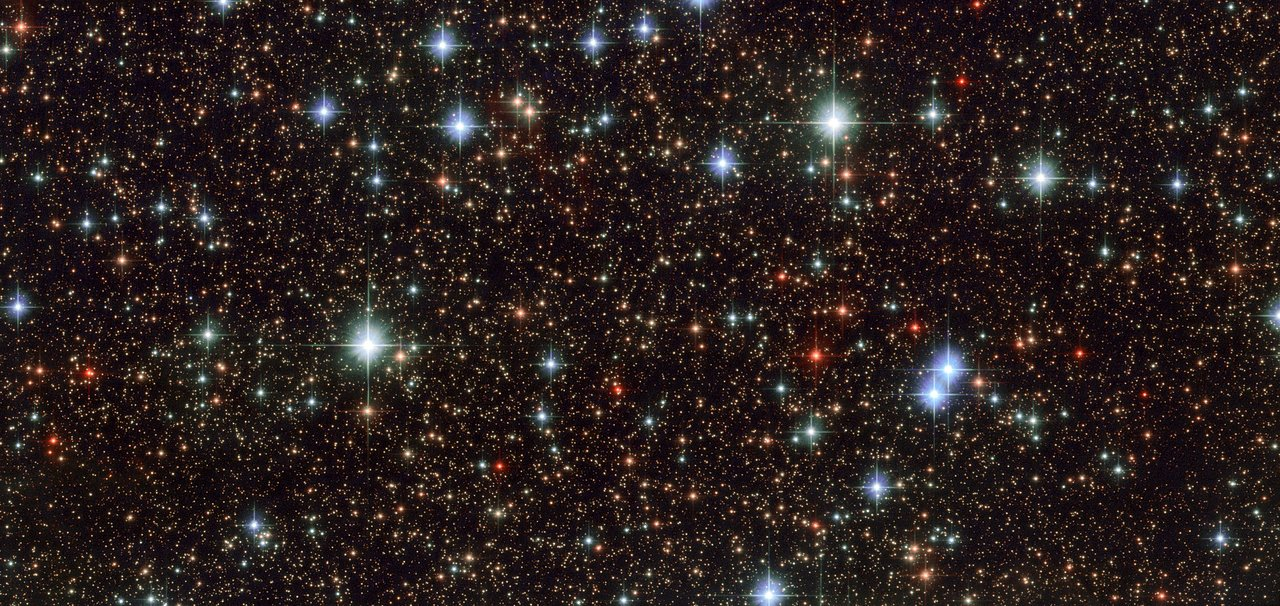
\includegraphics[width=0.9\textwidth]{prelim/hubble_friday_06172016}
  \caption{Hubble Space Telescope image of stars in the constellation Sagitarius. {\it Image credit: NASA/ESA.}}\label{f.hubblestars}
\end{figure}

Table \ref{t.spectralclass} lists the modern Harvard spectral types and some of their salient properties, including Main Sequence mass, radius, and luminosity.
Immediately apparent is the strong dependence of all these properties on the mass of the stars.
The most important parameter in determining the evolution of a star is its initial mass, usually termed as the Zero-age Main Sequence (ZAMS) mass.
But this is not the only important evolutionary parameter.
A stars {\it metallicity}, or content of elements heavier than H and He, as well as the initial angular momentum content and magnetic field strength are also critical.
These latter two are inextricably linked and subject to substantial uncertainties, both in their typical values for stars and in their impact on stellar evolution.
The roles of rotation and magnetic fields in stellar structure and evolution will be explored in Chapter \ref{ch.rotation}.
Another critical component in determining the fate of a star, particularly a massive star, is whether or not it has a close binary companion.
Important aspects of binarity will be discussed in Chapter \ref{ch.binaries}.


\begin{table}[hbt]
  \caption{The Modern Harvard Stellar Spectral Types}\label{t.spectralclass}
  \begin{tabular}{c|p{0.2\textwidth}p{0.2\textwidth}p{0.2\textwidth}p{0.2\textwidth}}
  \hline
  Type & Effective temperature & Main sequence mass & Main sequence radius & Main sequence bolometric luminosity \\
  \hline\hline
  O & $\gtrsim30,000$ K & $\gtrsim16\ M_\sun$ & $\gtrsim6.6\ R_\sun$ & $\gtrsim30,000\ L_\sun$ \\
  B & 10,000--30,000 K & 2.1--16 $M_\sun$ & 1.8--6.6 $R_\sun$ & 25--30,000 $L_\sun$ \\
  A & 7,500--10,000 K & 1.4--2.1 $M_\sun$ & 1.4--1.8 $R_\sun$ & 5--25 $L_\sun$ \\
  F & 6,000--7,500 K & 1.04--1.4 $M_\sun$ & 1.15--1.4 $R_\sun$ & 1.5--5 $L_\sun$ \\
  G & 5,200--6,000 K & 0.8--1.04 $M_\sun$ & 0.96--1.15 $R_\sun$ & 0.6--1.5 $L_\sun$ \\
  K & 3700--5200 K & 0.45--0.8 $M_\sun$ & 0.7--0.96 $R_\sun$ & 0.08--0.6 $L_\sun$ \\
  M & 2400--3700 K & 0.08--0.45 $M_\sun$ & $\lesssim$0.7 $R_\sun$ & $\lesssim$0.08 $L_\sun$ \\
  \hline
  \end{tabular}
\end{table}

The spectral classifications in Table \ref{t.spectralclass} are supplemented by {\it luminosity classes}, denoted by Roman numerals, with ``I'' being the brightest supergiants and ``V'' being main sequence stars.
The spectral classes are also typically augmented by and additional Arabic numeral further specifying the star's precise effective temperature.
So, for example, our Sun is a ``G2 V,'' being a main sequence star with an effective temperature of 5770 K.

\begin{figure}[htb]
  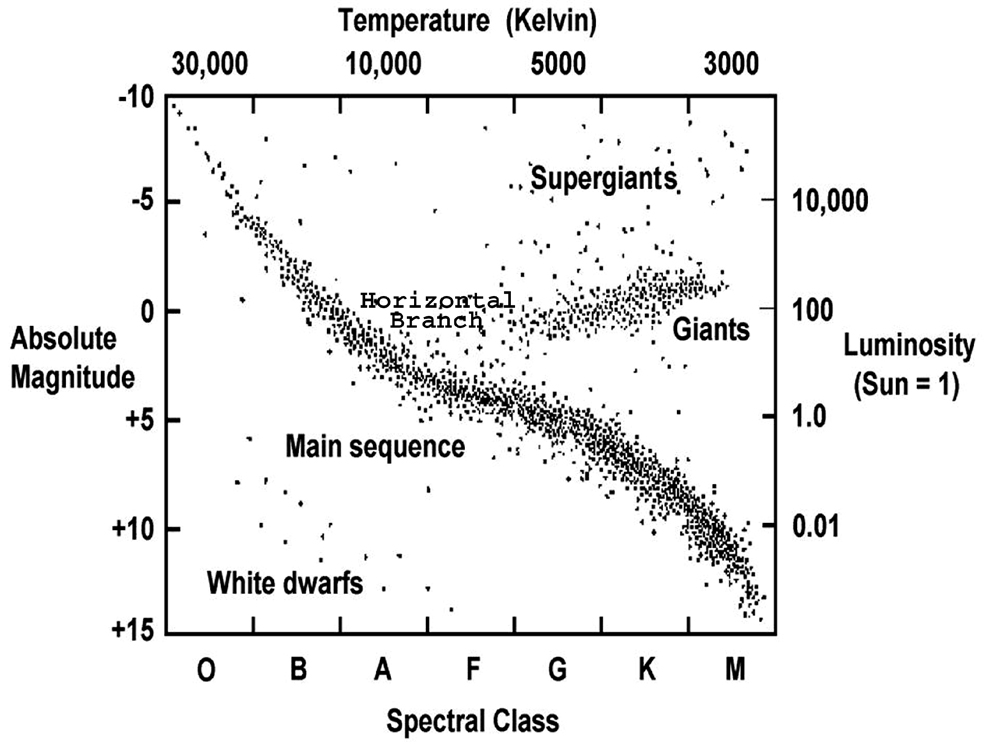
\includegraphics[width=0.9\textwidth]{prelim/HR_diagram}
  \caption{Example HR diagram for a subset of stars in the Milky Way.}
  \label{f.hrd}
\end{figure}

The principle graphical tool for understanding stellar evolution is the {\it Hertzprung-Russel (HR) diagram}.
Stars are placed on the HR diagram depending on their effective temperature (i.e., spectral type) and their absolute luminosity.
An example HR diagram is shown in Figure \ref{f.hrd}.
Observationally, it is generally easier to produce a {\it color-magnitude} diagram in which the absolute magnitude in a given broadband filter is plotted against the {\it color}, usually the difference of magnitudes between two broadband filters.


\chapter{The Sun on a Blackboard}\label{ch.introduction}
\input{introduction/introduction}

\chapter[Equations of Stellar Structure]{The Lagrangian Equations of Stellar Structure}\label{ch.stellar-structure-eqn}
% !TEX root = ../stellar-notes.tex

\section{The conservation laws}

After our rapid overview, we now gather the tools needed to tackle stellar evolution.  The first is to get the macroscopic equations for stellar structure. We will start from the equations expressing conservation of mass\footnote{In a relativistic system, we would instead start from conservation of baryon number, since mass is not invariant.}, momentum, and energy. We already derived the continuity (conservation of mass) equation,
\begin{equation}\label{e.mass-1}
\partial_{t}\rho + \divr(\rho\vu) = 0,
\end{equation}
and the Euler equation,
\begin{equation}\label{e.momentum-1}
\partial_{t}\vu + \vu\cdot\grad\vu = -\grad \Phi - \frac{1}{\rho}\grad P.
\end{equation}
Note that if we multiply eq.~(\ref{e.momentum-1}) by $\rho$, we can rewrite it, using eq.~(\ref{e.mass-1}), as
\begin{equation}\label{e.momentum-2}
	\partial_{t}(\rho\vu) + \divr[\vu(\rho\vu)] = -\rho\grad\Phi -\grad P.
\end{equation}
The left-hand side is interpreted as expressing the conservation of momentum ($\rho\vu$) in the absence of forces, analogous to eq.~(\ref{e.mass-1}) for the conservation of mass ($\rho$).

Note the general form of a conservation equation:
\begin{eqnarray*}
\lefteqn{\partial_{t}(\textrm{conserved quantity})}\\
 & & \mbox{} + \divr(\textrm{flux of conserved quantity}) =
 (\textrm{sources}) - (\textrm{sinks}).
\end{eqnarray*}
Because the momentum density $\rho\bvec{u}$ is a vector, its flux is a tensor: $[\bvec{u}(\rho\bvec{u})]_{ij} \equiv \rho u_{i}u_{j}$.\marginnote{By $\rho u_{i}u_{j}$, we mean the momentum along direction $i$ being transported along direction $j$.}

\newthought{The next equation is that of energy conservation.} Here we must consider both the internal energy per unit volume $E/V = \rho \varepsilon$ and the kinetic energy per unit volume $\rho u^{2}/2$.  In this section $\varepsilon$ represents the internal energy per unit mass of the fluid. In a fixed volume of the fluid the total energy is thus
\[ \int_{V} \left(\rho \frac{1}{2}u^{2} + \rho \varepsilon \right)\,\dif V. \]
The flux of energy into this volume will clearly include
\[ -\int_{\partial V}\left(\frac{1}{2}\rho u^{2} + \rho \varepsilon\right) \vu\vdot\dif\bvec{S}. \]
But wait, there's more!  In addition, we have a conductive heat flux $\bvec{F}$; the total heat conducted through the surface $\partial V$ is
\[-\int_{\partial V}\bvec{F}\vdot\dif\bvec{S}.\]
Moreover, the pressure acting on fluid flowing into our volume does work on the gas at a rate
\[-\int_{\partial V}P\vu\vdot\dif\bvec{S}.\]
As a result, the net change of energy in our volume is
\begin{eqnarray}
\lefteqn{\partial_{t}\int_{V}\left(\frac{1}{2}\rho u^{2} + \rho \varepsilon\right)\nsp\dif V = }\nonumber \\
 && -\int_{\partial V} \!\dif\bvec{S}\vdot\left[\vu\left(\frac{1}{2}\rho u^{2} + \rho \varepsilon + P\right) + \bvec{F}\right] \nonumber\\
 &&+ \int_{V} \left( \rho \vu\vdot\bvec{g} + \rho q\right)\dif V.
\label{e.energy-1}
\end{eqnarray}
On the right-hand side we've added in the work done by gravity and the heating evolved by nuclear reactions (this could also involve sinks, such as neutrinos with a long mean free path).
Expressed in differential form, equation~(\ref{e.energy-1}) is
\begin{equation}\label{e.energy-2}
 \partial_{t}\left(\frac{1}{2}\rho u^{2} + \rho \varepsilon\right)
 	+ \divr\left[\rho\vu\left(\frac{1}{2} u^{2} + \varepsilon + \frac{P}{\rho}\right)\right]
	+ \divr\bvec{F} = \rho q + \rho \vu\vdot\bvec{g}.
\end{equation}
You are possibly wondering why I didn't put gravity, which can be expressed as a potential, on the left hand side of this equation.  The reason is that the gravitational stresses cannot be expressed in a  \emph{locally} conservative form; it is only when integrating over all space that the conservation law appears.

\newthought{Equations~(\ref{e.mass-1}), (\ref{e.momentum-2}), and (\ref{e.energy-2}) are supplemented by an equation of state,} which allows one to get from the pressure $P$, the temperature $T$, and the mass fractions $X_{i}$ of the species present, the remaining thermodynamical quantities, such as mass density $\rho$ and specific energy $\varepsilon$. In addition, Poisson's equation
\begin{equation}\label{e.poisson}
\nabla^{2}\Phi = 4\pi G\rho,
\end{equation}
specifies the gravitational acceleration $\bvec{g} = -\grad\Phi$. We then need one more equation to specify the heat flux $F$. We argued in \S\ref{s.energy-transport-estimate} that the typical length over which a photon travels before scattering is very small compared to the lengthscale over which the macroscopic properties of the star vary.  In this case, we expect the flux to obey a conduction equation of the form
\begin{equation}\label{e.conduction-simple}
\bvec{F} = -K\grad T.
\end{equation}
This assumption is clearly questionable near the stellar surface, and we have left unspecified the form of $K$.  Such an equation does, however, close the system of equations; all of the physics is then contained in the equation of state $P(\rho,T,\{X_{i}\})$, the rate of heating from nuclear reactions $q(\rho, T, \{X_{i}\})$, and the thermal conductivity $K(\rho,T,\{X_{i}\})$. Here $\{X_{i}\}$ are the mass fractions of the isotopes composing the solar plasma. We will also need a system of equations to describe how the $X_{i}$ change as a result of nuclear reactions and diffusion.


\section[Thermodynamics of a Mixture]{Thermodynamics of a mixture: A digression}\label{s.composition}
\subsection{Specifying the composition}
In this section we'll look at how one describes the composition for a multi-component plasma.  To make things concrete, let's imagine a box containing a mixture of nuclei, of many different isotopes, and electrons.  (To keep things simple, we'll assume complete ionization.)  Each isotope species $i$ has $N_{i}$ nuclei present, and is characterized by charge number $Z_{i}$ and nucleon number $A_{i}$.  Charge neutrality then specifies the number of electrons,
\begin{equation}\label{e.number-e}
N_{\mathrm{e}} = \sum_{i} Z_{i} N_{i}.
\end{equation}
The total mass of the box is
\begin{equation}\label{e.total-mass}
M = \me N_{\mathrm{e}} + \sum_{i} m_{i}N_{i},
\end{equation}
where $\me$ and $m_{i}$ are respectively the mass of an electron and a nucleus of species $i$.  Now what is $m_{i}$? Breaking a nucleus $i$ into $Z_{i}$ protons and $A_{i}-Z_{i}$ neutrons takes a certain amount of energy, the \emph{binding energy} $B_{i}$.  We can therefore write $m_{i} = Z_{i}\mpr + (A_{i}-Z_{i})\mn - B_{i}/c^{2}$, where $\mpr$ and $\mn$ are respectively the proton and neutron rest masses.

Inserting our expression for $m_{i}$ into equation~(\ref{e.total-mass}), dividing by the volume of the box $V$, and rearranging terms gives us the mass density,
\begin{equation}\label{e.rho}
\rho = \frac{M}{V} = \sum_{i} n_{i}\left[ \left(A_{i}-Z_{i}\right) \mn + Z_{i}\left(\mpr + \me\right) - B_{i}/c^{2}\right].
\end{equation}
Here $n_{i}$ is the number density of isotope species $i$, and we have used equation~(\ref{e.number-e}) to eliminate $N_{\mathrm{e}}$.  The numbers $n_{i}$ are, of course, fantastically\sidenote{astronomically?} large, so we scale the numbers by \emph{Avogadro's constant},
\begin{equation}\label{e.avogadro-def}
\NA = 6.0221367\ee{23}\nsp\unitstyle{mol}^{-1}.
\end{equation}
\marginnote{Recall that a \textbf{mole} is an amount of something: in $1\nsp\unitstyle{mol}$ there are $\NA$ items.}
If we multiply and divide the right-hand side of equation~(\ref{e.rho}) by $\NA$, we then have
\begin{equation}\label{e.molar-1}
\rho = \sum_{i} \left(\frac{n_{i}}{\NA}\right) \mathcal{A}_{i},
\end{equation}
where
\begin{equation}\label{e.gm-mol}
\mathcal{A}_{i} = \left[ \left(A_{i}-Z_{i}\right) \mn + Z_{i}\left(\mpr + \me\right) - B_{i}/c^{2}\right]\times\NA
\end{equation}
is the \emph{gram-molecular weight} of species $i$ with dimensions $[\mathcal{A}]\sim[\gram\cdot\mol^{-1}]$. Strictly speaking, the gram-molecular weight actually refers to the mass of a mole of the isotope in \emph{atomic} form; the right-hand side of eq.~(\ref{e.gm-mol}) is the gram-molecular weight neglecting the electronic binding energy.

Now you may wonder where the numerical value of $\NA$ came from.  It is not pulled out of thin air, but rather is defined so that \val{1}{\mol} of \carbon\ has a mass of exactly \val{12}{\gram}.  In other words, for \carbon\, $\mathcal{A} \equiv A\nsp\gram\usp\mol^{-1}$.  In fact for all nuclei, $\mathcal{A} \approx A \usp\gram\nsp\mol^{-1}$ to better than about 1\%, as demonstrated in Table~\ref{t.gm-mol}.
Because in CGS $\mathcal{A}\approx A$, it is customary to write $\mathcal{A} = A\times (1\usp\gram\nsp\mol^{-1})$, so that equation~(\ref{e.molar-1}) is
\begin{equation}\label{e.molar-2}
\rho = \sum_{i} \left(\frac{n_{i}}{\NA}\times 1\frac{\gram}{\mol}\right) A_{i}.
\end{equation}
This only works if our unit of mass is the gram: in SI units \carbon\ has a mass of $0.012\nsp\kilo\gram\usp\unitstyle{mol}^{-1}$.
Equation~(\ref{e.molar-2}) would be exact if $A$ were a real number, but the custom is to just keep it as the nucleon number, which introduces an error of order one percent. Astronomers typically then \emph{redefine} $\NA$ to mean $\NA(\textrm{astronomy})\equiv \NA / (1\nsp\gram\usp\mol^{-1}) = 6.0221367\ee{23}\nsp\gram^{-1}$. Alternatively, one can use the atomic mass unit (symbol $\amu$) defined as $1/12$ the mass of an atom of \carbon, so that $1\nsp\amu =  (1\nsp\gram\usp\mol^{-1})/\NA = 1.66054\ee{-24}\nsp\gram$. This puts equation~(\ref{e.molar-2}) into the more obvious form $\rho = \sum n_{i}\times A_{i}\mb$, with $\mb$ having a mass of $1\nsp\amu$.

\begin{table}[htbp]\caption{\label{t.gm-mol}Selected gram-molecular weights.}
\begin{center}
\begin{tabular}{r|ccc}
\hline
nuclide & $A$ & $\mathcal{A}$ & $(|\mathcal{A}-A|/A) \times 100$\\
\hline\hline
\neutron & 1 & 1.00865 & 0.865\\
\hydrogen & 1 & 1.00783 & 0.783\\
\helium & 4 & 4.00260 & 0.065\\
\oxygen & 16 & 15.99491 & 0.032\\
\silicon & 28 & 27.97693 & 0.082\\
\iron & 56 & 55.93494 & 0.116\\
\hline
\end{tabular}\end{center}
\end{table}

With the redefinition of \NA, equation~(\ref{e.molar-2}) can be rewritten as
\begin{equation}\label{e.}
1 = \sum_{i}\left(\frac{n_{i}}{\NA\rho}\right)A_{i} \equiv \sum_{i}Y_{i}A_{i}
\end{equation}
where $Y_{i} \equiv n_{i}/(\rho\NA)$ is the \emph{molar fraction}. It is customary to call $Y_{i}A_{i}$ the \emph{mass fraction} $X_{i}$, with $\sum X_{i} = 1$. We can then define the mean atomic mass number,
\begin{equation}\label{e.mean-A}
\bar{A} = \frac{\sum A_{i}Y_{i}}{\sum Y_{i}} = \frac{1}{\sum Y_{i}},
\end{equation}
and mean charge number
\begin{equation}\label{e.mean-Z}
\bar{Z} = \frac{\sum Z_{i}Y_{i}}{\sum Y_{i}} = \bar{A} \sum Z_{i}Y_{i}.
\end{equation}
The molar fraction of electrons is
\begin{equation}\label{e.Ye}
Y_{e} = \sum Z_{i} \frac{n_{i}}{\rho\NA} = \sum Z_{i}Y_{i} = \frac{\bar{Z}}{\bar{A}}.
\end{equation}
In stellar structure work, it is common to use the \emph{mean molecular weight}, defined so that the total number of particles, including electrons, per unit volume is
\begin{equation}\label{e.mean-molecular-weight}
\sum_{i} n_{i} + n_{e} \equiv \frac{\rho\NA}{\mu}.
\end{equation}
Yes, this is still the redefined $\NA$: $\mu$ is dimensionless. From the definition,
\begin{equation}
\mu = \left(\sum_{i}Y_{i} + Y_{e}\right)^{-1} = \left[ \sum_{i}\left(Z_{i}+1\right)Y_{i} \right]^{-1};\label{e.meanmol}
\end{equation}
sometimes astronomers also define the mean ion molecular weight, $\mu_{I} = (\sum Y_{i})^{-1}$, and the mean electron weight, $\mu_{e} = Y_{e}^{-1}$.

\begin{exercisebox}[Mean molecular weight of a hydrogen-helium plasma]
Consider a gas of \hydrogen\ and \helium\ with molar hydrogen fraction $Y_{\mathrm{H}}$.  Derive expressions for the molar fraction of \helium, $Y_{\mathrm{He}}$, $\bar{A}$, $\bar{Z}$, and $\mu$. What are the numerical value of these quantities for $Y_{\mathrm{H}} = 0.7$, i.~e., solar?
\end{exercisebox}

\begin{exercisebox}[Sound speed and kinetic energy of an ideal gas]
Assume that we can describe this plasma as an ideal gas.  What is the sound speed and the average kinetic energy of a particle, for a given mass density and temperature?
\end{exercisebox}


%In Ch.~\ref{ch.introduction} we listed the abundances of several elements in the sun: for $A_{\mathrm{el}} \equiv \log_{10}[N_{\mathrm{el}}/N_{\mathrm{H}}]+12$, $A_{\mathrm{H}} = 12.00$, $A_{\mathrm{He}} = 10.93$, $A_{\mathrm{N}}=7.78$, $A_{\mathrm{O}}=8.66$, $A_{\mathrm{C}} = 8.39$.  Assume that the isotopes for each element are, respectively, \hydrogen, \helium, \nitrogen, \oxygen, and \carbon; from this, derive the corresponding mass fractions for each isotope.

\section{The Equation of State of an Ideal Gas} \label{s.idealgas}
Equations~(\ref{e.mass-1}), (\ref{e.momentum-2}), and (\ref{e.energy-2} must be closed by a suitable {\it equation of state} that relates the thermodynamic quantities to each other.
A simple equation of state is that of an ideal gas.
An {\it ideal gas} is assumed to be made of vast numbers of point-like particles that interact only via elastic collisions.
This is generally a pretty good approximation for a monatomic, single-species gas but also works fairly well for molecular real gasses such as the terrestrial atmosphere, within certain limits.
Typically, a gas behaves more ideal at higher temperatures at which the kinetic motion of the particles dominate any intermolecular forces (i.e., van der Waals) that the gas may experience.
Ideal gasses obey the {\it ideal gas law}.
A {\it perfect gas} is a special case of an ideal gas that has constant specific heat capacities at constant volume and at constant pressure (see Section \ref{s.thermodynamics}).
In general, an ideal gas can have specific heat capacities that temperature- and/or density-dependent.

Consider a closed volume containing a large number of point-like collisional particles.
Elastic collisions of these particles with the walls of the volume will result in a force exerted on the walls.
In the absence of any external forces (i.e., gravity), the force exerted will be the same for all the walls of the volume.
The force per wall area is the {\it pressure} P on the walls.

The ideal gas law was first determined empirically by chemists in the 19th century and relates the pressure of a gas to its volume and temperature:
\begin{equation}
	PV = N_m R T, \label{e.ideal1}
\end{equation}
where $V$ is the volume of the gas, $T$ its temperature, $N_m$ the number of {\it moles} of gas, and $R$ is the universal gas constant.
It turns out, experimentally, the number of particles in a mole of gas is a universal constant: Avogadro's number \NA.
The universal gas constant is the product of Avogadro's number and the Boltzmann constant \kB: $R=\NA \kB$.
Thus, we can write the ideal gas law in a form more familiar to physicists,
\begin{equation}
	P = n\kB T,\label{e.ideal2}
\end{equation}
where $n = N_M\NA/V$ is the number density of particles in the gas.

If the particles can be described by a mean atomic mass $\bar{A}$ (Eq. \ref{e.mean-A}) then we can express the mass density in terms of the number density as $\rho = n A \mb$, where \mb is the atomic mass unit. Then another form of the ideal gas law is
\begin{equation}
	P = \frac{\rho}{\bar{A} \mb} \kB T.\label{e.ideal3}
\end{equation}

For a mixture of different particle types, including free electrons as we would have in a stellar plasma, we can express the ideal gas law in yet another equivalent form using the mean molecular weight,
\begin{equation}
	P = \frac{\NA \rho}{\mu} \kB T = \frac{\rho}{\mu \mb} \kB T,\label{e.ideal4}
\end{equation}
where we recognize that $\NA \approx \mb^{-1}$.
Using the definition of the mean molecular mass in terms of the molar fractions (Eq. \ref{e.meanmol}), we see that the total pressure is the sum of partial pressures,
\begin{equation}
	P = \left(\sum_{i}Y_{i} + Y_{e}\right) \NA \kB \rho T.\label{e.ideal5}
\end{equation}

Equations (\ref{e.ideal1}-\ref{e.ideal5}) are all equivalent for a gas of identical particles, with Eqs. (\ref{e.ideal4}) and (\ref{e.ideal5}) being more general for a mixture that includes free electrons as well as ions.

\section{Thermodynamics of Stellar Plasmas} \label{s.thermodynamics}

\subsection{The First Law}
Consider a volume of gas that can exchange energy with its surrounding either by the transfer of heat or by doing {\it work}.
Now assume the gas undergoes a truly {\it reversible} process, in which the state of the gas changes slowly enough that it is always in equilibrium.
I.e., throughout the entire process the gas moves through a series of infinitesimally different equilibrium states.
In such a process, the change in the gas internal energy will be
\begin{equation}
	\dif E = \dif Q - \dif W,
\end{equation}
where $dQ$ is the heat gained or lost and $dW$ is the work done {\it by} the gas (positive sign) or {\it on} the gas by its surroundings (negative sign).

First, let's consider how to deal with the work term.
If the gas is ``contained'' within some volume $V$, the gas exerts a differential force on the ``wall'' of this volume,
\[
	\delta \bvec{F} = P \delta A \hat{n},
\]
where $\delta A$ is some differential area element of the volume walls.
Now consider that the force exerted by the gas causes an infinitesimal displacement $\dif \bvec{x}$ in the volume walls doing some differential {\it work} (i.e., force through a distance),
\[
	\delta (\dif W) = \delta \bvec{F}\cdot\dif\bvec{x} = P (\hat{n}\cdot\dif\bvec{x})\delta A = P \delta V.
\]
Now, integrating over all area of the volume walls gives us $\dif W = P\dif V$, which you will recall elementary dynamics.
Then we have the First Law of Thermodynamics,
\begin{equation}
	\dif E = \dif Q - P\dif V. \label{e.first-law-extensive}
\end{equation}
\marginnote{First Law of Thermodynamics}

In Eq. (\ref{e.first-law-extensive}) the energy $E$ and heat $Q$ are {\it extensive} quantities that scale with the number of particles $N$ in our sample. In a fluid, however, these quantities are all functions of position. By $E(r)$, we mean that we can define a small portion of the star about the coordinate $r$ that is large enough particles to ensure that quantities such as pressure and temperature are well-defined, but small enough that we can treat $E(r)$ as a continuous function of position when integrating over the whole star.
\marginnote{Extensive vs. intensive quantities}

Using extensive quantities in fluid mechanics is cumbersome, so we instead use quantities like the energy per unit mass $\varepsilon  = E/(\rho V)$ or the heat per unit mass $q = Q/(\rho V)$. Since a fixed mass of fluid $M$ occupies a volume $V = M/\rho$, we can divide the first law, eq.~(\ref{e.first-law-extensive}), by $M$ to obtain
\begin{equation}\label{e.first-law-intensive}
\dif \varepsilon = \dif q - P\dif\left(\frac{1}{\rho}\right) = \dif q + \frac{P}{\rho^{2}}\dif \rho.
\end{equation}
The other extensive variables can be re-defined into mass-specific forms in a similar fashion.

The definition of an {\it adiabatic} process is one in which there is no change in the heat content of the system, $\dif Q \equiv 0$.
\marginnote{Adiabatic process}
Consider the Joule-Kelvin experiment in which a gas is allowed to expand adiabatically ($\dif Q=0$) into a larger volume initially a vacuum (i.e., $V_1 < V_2$).
Since the gas experiences no resistance while expanding into the new volume it does not do any work while expanding, $\dif W = P\dif V = 0$.
Therefore, by the First Law (Eq. \ref{e.first-law-extensive}), we have $\dif E = 0$ implying that the temperature remains constant during the expansion, $T_2 = T_1$.
Thus, the internal energy of the gas is a function only of temperature, $E(T)$.
In general, we would expect that the internal energy is also a function of density (or volume), $E(V,T)$.
This somewhat surprising result only holds for perfect gasses.

\subsection{Heat Capacity and Thermodynamic Derivatives}

Now consider a non-adiabtic process in which some heat, $\dif q$, is added to the system resulting in a temperature change $\dif T$.
The {\it specific heat capacity}, or simply specific heat, is then defined as
\[
	C \equiv \frac{\dif q}{\dif T},
\]
where, again, the heat per mass is $q$.
Specific heats are usually specified under conditions in which a thermodynamic quantity is assumed constant.
For instance, the specific heat at constant pressure is $C_P$ and the specific heat at constant volume is $C_V$.

A key feature of thermodynamics is that any thermodynamic quantity can be expressed as a function of any other {\it two} thermodynamic quantity.
Consider, for instance, the ideal gas law (e.g., Eq. \ref{e.ideal3}), which can obviously be arranged as we like to give $P(\rho, T)$, or $T(\rho, P)$, or $\rho(P,T)$.
Thus, it is useful to define derivatives of thermodynamic quantities with respect to others while keeping a third quantity fixed.
For variables $x, y, z$ we would write this using the notation,
\[
	\left(\frac{\partial z}{\partial x}\right)_y,
\]
where the subscript $y$ is the variable held fixed while calculating the derivative of $z$ with respect to $x$.

Now assume that our variables $(x,y,z)$ can be connected by some function $\mathcal{F}(x,y,z)=0$ (such as you might get by moving the RHS of the ideal gas law to the LHS).
Then, we can derive several useful relations (see Appendix \ref{s.thermo-derivatives}):
\begin{eqnarray}
	\left(\frac{\partial x}{\partial y}\right)_z &=& \frac{1}{(\partial y/\partial x)_z}, \\
	\left(\frac{\partial x}{\partial y}\right)_z \left(\frac{\partial y}{\partial z}\right)_x \left(\frac{\partial z}{\partial x}\right)_y &=& -1.
\end{eqnarray}
Now if some other quantity, $w$, is a function of any two of $(x,y,z)$, then
\begin{equation}
	\left(\frac{\partial x}{\partial y}\right)_w \left(\frac{\partial y}{\partial z}\right)_w = \left(\frac{\partial x}{\partial z}\right)_w.
\end{equation}

Consider as independent variables $(\rho, T, \varepsilon)$. Expanding the total differential of $\varepsilon$ in terms of its partial derivatives w.r.t. $\rho$ and $T$, we have
\[
	\dif \varepsilon = \left(\frac{\partial \varepsilon}{\partial T}\right)_\rho \dif T + \left(\frac{\partial \varepsilon}{\partial \rho}\right)_T \dif \rho.
\]
Using the First Law (Eq. \ref{e.first-law-intensive}) we then find
\begin{equation}
	\dif q = \left(\frac{\partial \varepsilon}{\partial T}\right)_\rho \dif T + \left[\left(\frac{\partial \varepsilon}{\partial rho}\right)_T - \left(\frac{P}{\rho^2}\right)\right] \dif \rho. \label{e.firstLaw2}
\end{equation}

For a process occurring at constant volume, the density is also constant\sidenote{Unless we are creating and destroying mass!}, $\dif \rho=0$.
The change in heat is given by $\dif q = C_V \dif T$.
Then by inspection, we find that the specific heat at constant volume is
\begin{equation}
	C_V = \left(\frac{\partial \varepsilon}{\partial T}\right)_\rho. \label{e.specHeatV}
\end{equation}
This is result is {\it completely general} for any thermodynamic expression relating $(\rho, T, e)$.

Similarly, at constant pressure the heat change is $\dif q = C_P \dif T$, and the specific heat is
\begin{equation}
	C_P = C_V + \left[\left(\frac{\partial \varepsilon}{\partial \rho}\right)_T - \left(\frac{P}{\rho^2}\right) \right] \left(\frac{\partial \rho}{\partial T}\right)_P. \label{e.specHeatP}
\end{equation}

For an adiabatic process, we have $\dif q = 0$ and can rearrange Eq. (\ref{e.firstLaw2}) to find
\begin{eqnarray}
		\left(\frac{\partial \varepsilon}{\partial T}\right)_\rho \dif T &+& \left[\left(\frac{\partial \varepsilon}{\partial \rho}\right)_T - \left(\frac{P}{\rho^2}\right)\right] \dif \rho = 0 \nonumber \\
		 \left(\frac{\partial \varepsilon}{\partial T}\right)_\rho \dif T &=& \left[\left(\frac{P}{\rho^2}\right) -\left(\frac{\partial \varepsilon}{\partial \rho}\right)_T \right] \dif \rho  \nonumber\\
		 \left(\frac{\partial \varepsilon}{\partial T}\right)_\rho \left(\frac{\partial T}{\partial \rho}\right)_s  &=& \left[\left(\frac{P}{\rho^2}\right) -\left(\frac{\partial \varepsilon}{\partial \rho}\right)_T \right] \nonumber\\
		 C_V \left(\frac{\partial T}{\partial \rho}\right)_s  &=& \left[\left(\frac{P}{\rho^2}\right) -\left(\frac{\partial \varepsilon}{\partial \rho}\right)_T \right]
\end{eqnarray}
where we have used the definition of the specific heat at constant volume (Eq. \ref{e.specHeatV}) and transformed the full derivative $(\dif T/\dif \rho)$ into a partial derivative at constant entropy, $s$.

The specific heat at constant pressure, Eq. (\ref{e.specHeatP}), is not nearly as simple and neat an expression as that for constant volume, Eq. (\ref{e.specHeatV}).
We can gain some physical insight into the specific heat at constant pressure by defining the specific {\it enthalpy}:
\begin{equation}
	h = \varepsilon + PV = \varepsilon + \frac{P}{\rho}.
\end{equation}
The change in enthalpy in some thermodynamic process is then
\[
	\dif h = \dif \varepsilon + P \dif(1/\rho) + \dif P / \rho
\]
Substituting into the First Law, Eq. (\ref{e.first-law-intensive}), we find
\[
	\dif q = \dif h - \frac{\dif P}{\rho}.
\]
Therefor, at constant pressure ($\dif P=0$) we recognize that we can write the specific heat by replace $q$ with $h$:
\begin{equation}
	C_P = \left(\frac{\partial h}{\partial T}\right)_P,
\end{equation}
a much simpler expression than Eq. (\ref{e.specHeatP}).
This implies that for isobaric processes, the enthalpy takes the role of internal energy for isovolumetric processes. \marginnote{Neat!}

\subsection{The Second Law}

Empirically, it is found that not all energy-conserving cyclic processes are possible.
That is, energy in such processes is transferred into, e.g., its surroundings and is rendered unavailable to do work or heat.
In a sense, the original energy of they system is {\it degraded} and, even if total energy is conserved, it is not possible to return the system to its original state.\marginnote{The process is irreversible.}

To understand this behavior of gasses, we must first introduce a new thermodynamic state function, {\it entropy} $S$.
If in a reversible process a system exchanges some heat $\dif Q$ with a reservoir at temperate $T$, the than change in entropy is
\begin{equation}
	\dif S \equiv \frac{\dif Q}{T}. \label{e.difS}
\end{equation}
Using this definition of entropy, we can re-write the First Law (Eqs. \ref{e.first-law-extensive} and \ref{e.first-law-intensive}) as
\begin{eqnarray}
	T \dif S = \dif E + P \dif V \\
	T \dif s = \dif \varepsilon + \frac{P}{\rho^2}\dif\rho,
\end{eqnarray}
where the second version is the intensive form as we have entropy the {\it specific entropy} $s$.

For any cyclic process, the integral of Eq. (\ref{e.difS}) over an entire cycle must to be less than equal to zero. That is
\begin{equation}
	\oint \frac{\dif Q}{T} \leq 0. \label{e.sec-law-1}
\end{equation}
This is an elementary state of the Second Law of Thermodynamics.

To elucidate the meaning of this further, consider a reversible process in which heat $\dif Q_1 (T)$ is delivered to the system.
In order to reverse the process and return the system to its original state, heat $\dif Q_2 (T) \equiv -\dif Q_1 (T)$ must be given to the system. Equation (\ref{e.difS}) requires that any cycle of the system satisfies both
\[
	\oint \frac{\dif Q_1 (T)}{T} \leq 0
\]
and
\[
	\oint \frac{\dif Q_2 (T)}{T} = -\oint \frac{\dif Q_1(T)}{T} \leq 0.
\]
In order for both conditions to be simultaneously true, the heat transfer must be zero so that for a reversible process
\begin{equation}
	\oint_\mathrm{rev} \frac{\dif Q}{T} = 0. \label{e.rev-dQ}
\end{equation}
This then implies that $\dif S = 0$ by Eq. (\ref{e.difS}).
I.e., in a reversible process, the entropy remains constant.

It will turn out that Eq. (\ref{e.difS}) is an {\it exact} differential, i.e. $\int dS$ is path-independent.\marginnote{An exact differential is one that can be express $\dif f = (\partial f / \partial x)_y \dif x + (\partial x / \partial y)_x \dif y$.}
In other words, the entropy difference between two states is independent of the details of the reversible process connecting them.
If $A$ and $B$ are two states connected by a reversible cycle made up of path 1 ($A$ to $B$) and path 2 ($B$ to $A$) then Eq. (\ref{e.rev-dQ}) implies
\begin{equation}
	\oint \frac{\dif Q}{T} = \left(\int_A^B\frac{\dif Q}{T}\right)_1 + \left(\int_B^A\frac{\dif Q}{T}\right)_2 = 0.
\end{equation}
Now that we've specified some limits we can write these integrals in terms of the entropies of the states via Eq. (\ref{e.difS})
\[
	\left(\int_A^B\frac{\dif Q}{T}\right)_1 = S(B) - S(A),
\]
which gives us
\begin{equation}
	S(B) - S(A) = -\left(\int_B^A\frac{\dif Q}{T}\right)_2 = \left(\int_A^B\frac{\dif Q}{T}\right)_2,
\end{equation}
which proves that the entropy difference of the states doesn't depend on the details of the processes.

Now let's consider that an {\it irreversible} process $I$ connects $A$ to $B$ then reversible process $R$ returns $B$ to $A$.
Now via Eq. (\ref{e.sec-law-1})
\begin{equation}
	\int_I \frac{\dif Q}{T} + \int_R\frac{\dif Q}{T} \leq 0,
\end{equation}
or
\begin{equation}
	\int_I \frac{\dif Q}{T} \leq \left(-\int_B^A\frac{\dif Q}{T}\right)_R = \left(\int_A^B\frac{\dif Q}{T}\right)_R = S(B) - S(A).
\end{equation}
This implies that for an isolated system (i.e., $\dif Q=0$) entropy can only increase:
\[
	S(B) \geq S(A)
\]
where the equality holds for reversible processes only.
All processes in the real world are actually irreversible, at least to some extent.
Thus, the entropy of any real system always increases, even if that system is perfectly thermally insulated ($\dif Q=0$).

\subsection{Some Thermal Properties of Ideal Gasses}

We often approximate stellar plasmas as ideal gasses, fraught as that may be.
As we argued above, the internal energy is a function of temperature only.
So using the definition of the specific heat (Eq. \ref{e.specHeatP}) we have
\begin{equation}
	\varepsilon = \int C_V \dif T.
\end{equation}
While the proof will require some more development of kinetic theory, we will find that $C_V$ is a constant for an ideal gas, thus
\begin{equation}
	\varepsilon = C_V T.
\end{equation}



\section{The equations in Lagrangian form}

The fluid equations~(\ref{e.mass-1}), (\ref{e.momentum-2}), and (\ref{e.energy-2}) are in \textbf{Eulerian} form; that is, they describe everything in terms of spatial coordinates and time. This is not necessarily the most convenient form for  practical calculations. For example, the star can expand and contract, making the radius a function of time. Moreover, the velocity $\vu$ is \emph{not} the velocity of a given fluid element, which is why the equation of motion (eq.~[\ref{e.euler}]) is non-linear. It is often desirable to put the fluid equations into \textbf{Lagrangian} form, in which the coordinates are some label for a fluid element and time.

In one-dimension, the transformation to Lagrangian equations is easy.  At some reference time, we label the mass enclosed by a shell of radius $r$
\begin{equation}\label{e.mass}
	m(r,t) = \int_{0}^{r}\! \rho(r',t) 4\pi r'^{2} \,\dif r',
\end{equation}
as a Lagrangian coordinate $m$; we then transform coordinates from $(r,t)$ to $(m,t)$.
To do this, differentiate eq.~(\ref{e.mass}) w.r.t.\ $r$,
\[ \partial_{r}m = 4\pi r^{2}\rho, \]
and substitute for $\rho$ in the equation of  continuity (eq.~[\ref{e.mass-1}]).  The first term becomes
\[
	\partial_{t}\rho = \partial_{t}\left(\frac{1}{4\pi r^{2}} \partial_{r} m\right)
	= \frac{1}{4\pi r^{2}}\partial_{r}(\partial_{t}m),
\]
while the second term becomes
\[
	\frac{1}{4\pi r^{2}}\partial_{r}\left(u\partial_{r}m\right);
\]
the equation of continuity therefore becomes
\begin{equation}\label{e.mod-continuity}
	\frac{1}{4\pi r^{2}} \partial_{r}\left( \partial_{t} m + u\partial_{r} m\right) = 0.
\end{equation}
We can integrate this over $r$ to find that $\partial_{t} m + u\partial_{r} m = f(t)$, where $f(t)$ is some as-yet-unspecified function; to fix $f(t)$, we note that since $m(0,t) = 0,\;\forall t$, we must have $f(t) = 0$.  Now $\partial_{t} m + u\partial_{r} m = \Dif m/\Dif t = 0$, so along a streamline, $m$ is a constant.  We can therefore transform from coordinates $(r,t)$ to $(m,t)$ by setting
\begin{eqnarray}
	\label{e.lagrange-rule-1}
	\left.\frac{\partial}{\partial_{t}}\right|_{r} + u\left.\frac{\partial}{\partial r}\right|_{t}
	&=& \left.\frac{\partial}{\partial t}\right|_{m} \equiv \frac{\Dif}{\Dif t}\\
	\label{e.lagrange-rule-2}
	\left.\frac{\partial}{\partial r}\right|_{t} &=& 4\pi r^{2}\rho \left.\frac{\partial}{\partial m}\right|_{t}.
\end{eqnarray}
Here $\Dif/\Dif t \equiv (\partial/\partial t)_{m}$ is the Lagrangian time derivative.  In deriving this change, we used the equation of continuity, which becomes
\begin{equation}\label{e.lagrange-r}
\frac{\partial r}{\partial m} = \frac{1}{4\pi r^{2}\rho}.
\end{equation}
Our equation for momentum (eq.~[\ref{e.momentum-1}]) becomes
\begin{equation}\label{e.lagrange-momentum}
\frac{\partial P}{\partial m} = -\frac{Gm}{4\pi r^{4}} - \frac{1}{4\pi r^{2}}\frac{\Dif u}{\Dif t}.
\end{equation}
In hydrostatic balance the second term on the right-hand side is negligible.
The flux equation, (eq.~[\ref{e.conduction-simple}]) can be transformed to
\begin{equation}\label{e.lagrange-flux}
\frac{\partial T}{\partial m} = - \frac{1}{16\pi^{2} r^{4}\rho K}L_{r}
\end{equation}
Here $L_{r}$ is the luminous flux at a radius $r$.
%	\frac{\partial T}{\partial m} = -\frac{3}{64\pi^{2}r^{4}}\frac{\kappa}{ac T^{3}}L_{r}.

The energy equation (eq.~[\ref{e.energy-2}]) is more complicated. We can expand the time derivative as
\begin{eqnarray*}
	\partial_{t} \left( \frac{1}{2}\rho u^{2} + \rho \varepsilon \right)
	&=& \left(\frac{1}{2}u^{2} + \varepsilon\right)\partial_{t}\rho + \rho\partial_{t}\left[\frac{1}{2}(\vu\vdot\vu) + \varepsilon\right]\\
	&=& -\left(\frac{1}{2}u^{2} + \varepsilon\right)\divr\left(\rho\vu\right) + \rho \vu\partial_{t}\vu + \rho\partial_{t}\varepsilon,
\end{eqnarray*}
using equation~(\ref{e.mass-1}) to substitute for $\partial_{t}\rho$.  We then use equation~(\ref{e.momentum-1}) to replace $\partial_{t}\vu$, and recognizing that $\vu(\vu\vdot\grad)\vu = \vu\vdot\grad[(1/2)u^{2}]$, rewrite equation~(\ref{e.energy-2}) as
\begin{equation}\label{e.energy-3}
	\rho\left(\partial_{t} + \vu\vdot\grad\right) \varepsilon + P\divr\vu = -\divr\bvec{F} + \rho q.
\end{equation}
We've canceled all common factors here.  Finally, we once again use equation~(\ref{e.mass-1}) to set
\[
	P\divr\vu = -(P/\rho)(\partial_{t}\rho + \vu\vdot\grad \rho)
	= \rho P\left(\partial_{t} + \vu\vdot\grad\right)\left(\frac{1}{\rho}\right).
\]
Substituting this into the left-hand of equation~(\ref{e.energy-3})  and using the first law of thermodynamics (see eq.~[\ref{e.first-law-intensive}]), we obtain
\begin{equation}
\rho\left(\partial_{t} + \vu\vdot\grad\right) \varepsilon + P\divr\vu = \rho T \left(\partial_{t} + \vu\vdot\grad\right) s.
\end{equation}
For the right-hand side of equation~(\ref{e.energy-3}), we expand the divergence operator in spherical symmetry and use equation~(\ref{e.lagrange-rule-2}) to obtain
\[
	-\divr\bvec{F} = -\frac{1}{r^{2}}\frac{\partial(r^{2} F)}{\partial r} = -\rho\frac{\partial L_{r}}{\partial m}.
\]
Putting everything together, we finally have our heat equation in Lagrangian form,
\begin{equation}\label{e.lagrange-heat}
	\frac{\partial L_{r}}{\partial m} = q - T\frac{\Dif s}{\Dif t}.
\end{equation}
This has a simple interpretation: the change in luminosity across a mass shell is due to sources or sinks of energy and the change in the heat content of the shell.

\begin{exercisebox}[Lagrangian form of $T\Dif s/\Dif t$]
 \label{p.lagrange-heat} Show that equation (\ref{e.lagrange-heat}) can be written as
\begin{eqnarray}
\frac{\partial L_{r}}{\partial m} &=& q - \frac{c_{\rho} T}{\chi_{T}}\left\{\frac{\Dif\ln P}{\Dif t} - \left[\chi_{\rho} + \chi_{T}\left(\Gamma_{3} - 1\right)\right]\frac{\Dif\ln \rho}{\Dif t}\right\}\\
 &=& q - \frac{P}{\rho(\Gamma_{3}-1)}\frac{\Dif }{\Dif t}\ln\left(\frac{P}{\rho^{\Gamma_{1}}}\right),
\label{e.lagrange-heat-alt2}
\end{eqnarray}
where
\begin{eqnarray*}
 \chi_{T} &\equiv& \frac{T}{P}\tderiv{P}{T}{\rho},\\
 \chi_{\rho} &\equiv& \frac{\rho}{P}\tderiv{P}{\rho}{T},\\
 \Gamma_{1} &\equiv& (\partial \ln P/\partial\ln \rho)_{s}\,,\textrm{and}\\
 \Gamma_{3}-1 &\equiv& \tderiv{\ln T}{\ln \rho}{s}
\end{eqnarray*}
are defined in Appendix~\ref{s.thermo-derivatives}.
\end{exercisebox}


It is more useful, however, to work with temperature and pressure instead of entropy.  Write
\[
	T\frac{\Dif s}{\Dif t} = T\tderiv{s}{T}{P}\frac{\Dif T}{\Dif t} + T\tderiv{s}{P}{T}\frac{\Dif P}{\Dif t},
\]
and use the identity (see Appendix~\ref{s.thermo-derivatives})
\[
	\tderiv{s}{P}{T} = -\tderiv{s}{T}{P}\tderiv{T}{P}{s}
\]
to obtain
\begin{equation}\label{e.lagrange-heat-alt}
	\frac{\partial L_{r}}{\partial m}
	= q - c_{P}\left[ \frac{\Dif T}{\Dif t} - \tderiv{T}{P}{s} \frac{\Dif P}{\Dif t}\right].
\end{equation}
Equations~(\ref{e.lagrange-r}), (\ref{e.lagrange-momentum}), (\ref{e.lagrange-flux}), and (\ref{e.lagrange-heat-alt}), when supplemented by an equation of state, a prescription for the thermal conductivity, and the equations for nuclear heating and neutrino cooling, form the equations for stellar structure and evolution in spherical symmetry.


\chapter[Polytropes]{Polytropes and the Lane-Emden Equation}\label{ch.polytropes}
\input{Lane-Emden/Lane-Emden}

\chapter[Kinetic Theory]{Kinetic Theory for Stars}\label{ch.kinetic}
%\input{}

\chapter{Radiation Transport}
% !TEX root = ../stellar-notes.tex

The sun is very opaque.  Were photons able to stream freely, they would exit in $\sim \Rsun/c = 2.0\nsp\second$.  Given the luminosity of the sun, however, we derived that the time  for the sun to radiate away its stored thermal energy is instead millions of years (see eq.~[\ref{e.K-H}]).  As a result, we can regard the sun as a cavity filled with photons with a very slight leakage.  This is the description commonly invoked to describe blackbody radiation, and we expect that in the interior of the sun, the radiation can be described by a photon gas in thermal equilibrium at the ambient temperature.

\section{Description of the Radiation Field}\label{s.radiation-description}

Consider a cavity containing a gas of photons. In general we can describe the mean number of photons in this cavity as
\begin{equation}\label{e.photon-occupation}
 N = \int f(\vp,\vx)\,\dif^{3}x\,\dif^{3}p.
\end{equation}
Here $f$ is a distribution function, as described in Chapter~\ref{ch.equation-of-state}; if we are in thermal equilibrium, $f$ is of course the Bose-Einstein distribution (cf.\ eq.~[\ref{e.boson-dist}]), but our discussion here will be more general.  Consider a small opening on our cavity with area $\dif A$ and unit normal $\unitn$.  The energy incident on this area in a time $\dif t$ having propagation vector along $\unitn$ and propagating into solid angle $\dif\Omega$ (see Fig.~\ref{f.intensity-schematic}) is found by integrating equation~(\ref{e.photon-occupation}) over a volume $\dif^{3}x = c\dif t\,\dif A$,
\[
\dif E = \dif A\,c\dif t\,\left( p^{2}\dif p\,\dif\Omega\right)  h\nu \, f.
\]
Since the photon momentum is $p = h\nu/c$, we have
\begin{equation}\label{e.specific-intensity}
I_{\nu} \equiv \frac{\dif E}{\dif t\,\dif A\,\dif\Omega\,\dif\nu} = \frac{h^{4}\nu^{3}}{c^{2}} f.
\end{equation}
This defines the \emph{specific intensity} $I_{\nu}$.  It is easy to show that in the absence of interactions with matter, $I_{\nu}$ is conserved along a ray (see, e.g., Rybicki \& Lightman).

If the photons are in thermal equilibrium, then $f$ is the Bose-Einstein distribution, $f = (2/h^{3})(\exp[h\nu/\kB T]-1)^{-1}$, and the specific intensity becomes
\begin{equation}\label{e.Bnu}
B_{\nu} \equiv \frac{2 h\nu^{3}}{c^{2}} \left[\exp\left(\frac{h\nu}{\kB T}\right)-1\right]^{-1}.
\end{equation}
Here $B_{\nu}$ is called the \emph{Planck function}.

\begin{marginfigure}
\includegraphics{intensity-schematic}
\caption{\label{f.intensity-schematic}Schematic of a pencil of radiation propagating into an angle $\dif\Omega$.}
\end{marginfigure}

The specific intensity plays the role of the {\it distribution function} for radiation.
We can similarly derive important physical quantities by taking moments of the specific intensity, but in angle rather than momentum space.
The {\it zeroth} moment of the specific intensity is
\begin{equation}
  J_\nu = \frac{1}{4\pi} \int I_\nu \dif\Omega,
\end{equation}
and is called the {\it mean intensity} as it is essentially an angle average of the specific intensity.


The energy density per frequency $u_{\nu}$ can be defined as $\dif E/(c \dif t\,\dif A\,\dif\nu)$, that is, the energy per unit frequency that is in a cylinder of length $c\,\dif t$ and cross-sectional area $\dif A$; comparing $u_{\nu}$ with the definition of $I_{\nu}$, we see that
\begin{equation}
  u_{\nu} = \frac{1}{c}\int I_{\nu}\,\dif\Omega = \frac{4\pi}{c} J_\nu.
\end{equation}
For a blackbody, $I_{\nu}=B_{\nu}$ doesn't depend on angle, and we can integrate over $\dif\Omega$,
\begin{equation}\label{e.radiation-energy-density}
u_{\nu}= \frac{8\pi h\nu^{3}}{c^{3}}\left[\exp\left(\frac{h\nu}{\kB T}\right)-1\right]^{-1}.
\end{equation}
The total energy density can then be found by integrating over all frequencies, giving
\[ u = \left[\frac{8\pi^{5}\kB^{4}}{15 h^{3}c^{3}}\right] T^{4}\equiv aT^{4} \]
in agreement with what we derived from statistical mechanics, \S\ref{s.relativistic-photon-gas}.

The next quantity to define is the \emph{flux} of energy, along direction $\unitk$, per unit time $\dif t$,  per unit area $\dif A$, and per frequency interval $\dif\nu$. We take the {\it first} moment of the specific intensity by multiplying $I_{\nu}$ by a direction vector $\unitk$ and integrating over $\dif\Omega$:
\begin{equation}\label{e.radiation-flux}
\bvec{F}_{\nu} = \int \unitk I_{\nu} \,\dif\Omega.
\end{equation}
Note that $\bvec{F}_{\nu}$ is a vector;   the net flux along a direction \unitn\ is
\[ F_{\nu} = \int I_{\nu}(\unitn\cdot\unitk)\dif\Omega. \]
If we take our polar angle with respect to $\unitk$, then $(\unitn\cdot\unitk)\,\dif\Omega = \cos\theta\,\sin\theta\,\dif\theta\,\dif \phi$; defining the direction cosine $\mu = \cos\theta$, this becomes
\[ F_{\nu} = \int I_{\nu} (\unitn\cdot\unitk)\,\dif\Omega = \int_{0}^{2\pi} \int_{-1}^{1} I_{\nu}\mu\,\dif\mu\,\dif\phi. \]
Note that if the radiation field is isotropic then $F_{\nu}=0$: there must be some anisotropy in the radiation field to generate a net flux.

For blackbody radiation, if we only integrate over outgoing directions, $0\le \mu\le 1$, as would be the case for thermal radiation emerging from a \emph{hohlraum},
\[ F_{\nu} = \pi B_{\nu}.\]
Integrating this $F_{\nu}$ over all frequencies, we recover the Stefan-Boltzmann formula,
\[ F = \left(\frac{ac}{4}\right) T^{4} \equiv \sigma_{\mathrm{SB}} T^{4}, \]
where $\sigma_{\mathrm{SB}}$ is the Stefan-Boltzmann constant.

Finally, let's look at the momentum flux along direction $\unitj$ being transported along direction \unitk, per unit time $\dif t$, per unit area $\dif A$, and per unit frequency interval $\dif\nu$.  Since for a photon, $E = pc$, we divide the energy flux by $c$.
This is a \emph{tensor},
\begin{equation}\label{e.radiation-pressure-tensor}
\btens{P}_{\nu} = \frac{1}{c}\int \unitj\unitk I_{\nu}\dif\Omega.
\end{equation}
This is just the {\it second} angular moment of the specific intensity.
The net (isotropic) momentum flux along a direction \unitn\ is then
\[ P_{\nu} = \frac{1}{c}\int (\unitn\cdot\unitk)(\unitn\cdot\unitk) I_{\nu}\,\dif \Omega = \frac{2\pi}{c}\int_{-1}^{1} I_{\nu}\mu^{2}\,\dif\mu. \]
For blackbody radiation,
\[ P_{\nu} = \frac{4\pi}{3c} B_{\nu}  = \frac{1}{3}u_{\nu}\]
and we may integrate this over frequency to obtain $P = u/3$, the standard result from thermodynamics.

\section{Some simple estimates}

We argued in the previous section that the solar interior is quite opaque. Naively, we might imagine some radiative transition, e.g. bremsstrahlung, emitting a photon.  The photon speeds away at $c$, but it doesn't get very far before being absorbed or scattered by another particle. A new photon, either due to emission or scattering, will be emitted at some random direction, and the whole process repeats. This is just a description of a \emph{random walk}.

For some simple estimate, let's assume that the hop is the same for all photons, regardless of frequency or ambient temperature. If the hop length is $\ell$, then we know that the total path length to get from the center to the surface is $\Rsun(\Rsun/\ell)$ and the time for this to occur is $\Rsun^{2}/\ell/c$. What is a good estimate for $\ell$?  Consider a planar electromagnetic wave incident on a collection of scatterers. If these scatterers are uncorrelated, then the probability of scattering is just the number of scatterers times the probability for scattering from a single scatterer.  Define the probability of scattering as
\begin{equation}\label{e.scattering-probability}
\mathcal{P} = N\times\left(\frac{\textrm{energy scattered per unit time by one scatterer}}{\textrm{energy incident per unit time per unit area}}\right)\frac{1}{ \mathcal{A}}
\end{equation}
where $\mathcal{A}$ is the area normal to the propagation direction \unitk\ of the volume containing the $N$ scatterers.  The quantity in parenthesis is just the definition of the cross-section $\sigma$. Furthermore, if we set $\mathcal{P} = 1$, then the total number of scatters is just $N = n\times \mathcal{A}\times \ell$, where $n$ is the number density of scatterers. Thus we define the \emph{mean free path},
\begin{equation}\label{e.mean-free-path}
\ell = \frac{1}{n\sigma}.
\end{equation}
In stellar work, it is more convenient to use mass density rather than number density.  Writing $n = Y\rho/\mb$, where $Y$ is the abundance of scatterers, we have
\[ \ell = \rho^{-1} \left(\frac{\mb}{Y\sigma}\right) \equiv (\rho\kappa)^{-1} \]
where $\kappa$ is the \emph{opacity} and has dimensions $[\kappa]\sim[\cm^{2}\nsp\gram^{-1}]$.

The opacity in the stellar interior is set by a large number of processes (see \S\ref{s.opacity-sources}): Thomson scattering, free-free absorption, atomic absorption, and photoionization.  In general, the cross-section depends on the ambient temperature and density and the frequency of the photon.
Over the length of a hop $\ell$ the temperature and density will only vary slightly.  As a result, the conditions are nearly isotropic, so we indeed expect the radiation to come into thermal equilibrium with the ambient material.  But the conditions are not perfectly isotropic---otherwise there would be zero net heat flux!  It is the small anisotropy that gives rise to the transport of energy.  Let's imagine a small cube of material, with the size of this cube being $\ell$.  Because we are so very nearly isotropic and in thermal equilibrium, the flux through any one face of this cube must be $(c/6)u$.  Now suppose we have two adjacent cubes, with the common face of the cubes being at $x=0$.  The flux across the face has contributions from photons emitted at $x-\ell$ and $x+\ell$, so the net flux is
\begin{eqnarray}
	F &\approx& \frac{c}{6} u(x-\ell) - \frac{c}{6} u (x+\ell)\nonumber \\
	&\approx& -\frac{1}{3}c\ell\frac{\dif u}{\dif x}.\label{e.rad-diffusion-simple}
\end{eqnarray}
This is a diffusion equation with coefficient $c/(3\rho\kappa)$.  Our derivation is very crude, as it neglects the variation in cross section with the properties of the ambient medium and with the photon frequency.  Nonetheless, this is basically the correct scenario; heat diffuses with a coefficient given by some suitably defined average over all sources of opacity.

\section{Equation of Transfer}

We're now ready to formalize the crude work in the previous section.
In the absence of interactions with matter, the specific intensity $I_{\nu}$ is conserved along a ray propagating in direction \unitk: $\dif I_{\nu}/\dif s = c^{-1}\partial_{t}I_{\nu} + \unitk\cdot\grad I_{\nu} = 0$. If matter is present, it can do three things to change $I_{\nu}$.
\begin{description}
\item[emit] Matter may spontaneously emit photons and add to the beam: $\dif I_{\nu}/\dif s = \rho\varepsilon_{\nu}/(4\pi)$. Here $\varepsilon_{\nu}$ is the energy spontaneously emitted per unit frequency per unit time per unit mass.  The factor of $4\pi$ is to make this term per steradian.

\item[absorb] Photons have a chance of being absorbed or scattered out of the beam: $\dif I_{\nu}/\dif s = -\rho\kappa_{\nu}I_{\nu}$. Here the right-hand side is the energy removed from the beam along a path $\dif s$ with $\kappa_{\nu} = \kappa_{\nu}^{\mathrm{abs}} + \kappa_{\nu}^{\mathrm{sca}}$ being the total opacity (absorption plus scattering). The dimensions of opacity are clearly $[\kappa_{\nu}] \sim [\cm^{2}/\gram]$. (If we had stimulated emission, this would be a \emph{negative} $\kappa_{\nu}$.)

\item[scatter] Photons may be scattered into the beam from other directions: $\dif I_{\nu}/\dif s = \rho\kappa_{\nu}^{\mathrm{sca}}\phi_{\nu}$. If the scattering is isotropic, then
\begin{equation}\label{e.isosca}
\phi_{\nu} = \frac{1}{4\pi}\int_{0}^{2\pi}\!\!\!\int_{0}^{\pi} I_{\nu}\,\dif\phi\,\sin\theta\,\dif\theta \equiv J_{\nu},
\end{equation}
where $J_{\nu}$ is the mean intensity: the scattering redistributes the energy over all angles.
\end{description}
Putting all these terms together gives us the \emph{equation of transfer},
\begin{equation}\label{e.transfer}
\frac{1}{c}\partial_{t}I_{\nu} + \unitk\cdot\grad I_{\nu} = \rho \frac{\varepsilon_{\nu}}{4\pi} - \rho\kappa_{\nu} I_{\nu} + \rho\kappa_{\nu}^{\mathrm{sca}}\phi_{\nu}
\end{equation}
for the specific intensity $I_{\nu}$.

\subsection{Radiative equilibrium}
The emissivity $\varepsilon_{\nu}$ and the opacity $\kappa_{\nu}$ describe how the radiation interacts with matter. A condition of steady-state is that the gas not gain or lose energy to the radiation. This requires balancing
\[ \left(\textrm{energy emitted per unit volume}\right) = \rho\int\frac{\varepsilon_{\nu}}{4\pi}\,\dif\nu\,\dif\Omega\]
with
\[ \left(\textrm{energy absorbed per unit volume}\right) = \rho\int \kappa_{\nu}^{\mathrm{abs}} I_{\nu}\,\dif\nu\,\dif\Omega,\]
or
\begin{equation}\label{e.rad-equil}
\int_{0}^{\infty}\! \left(\frac{\varepsilon_{\nu}}{4\pi} - \kappa_{\nu}^{\mathrm{abs}} J_{\nu}\right)\,\dif\nu = 0.
\end{equation}
Here we assume $\varepsilon_{\nu}$ does not depend on angle. We don't include scattering because it doesn't transfer energy between the radiation and the gas.

Now suppose that the level populations of the matter are in thermal equilibrium and can be described by a temperature $T$.  In that case, detailed balance must hold, so that
\begin{equation}\label{e.detail-balance}
\frac{\varepsilon_{\nu}}{4\pi\kappa_{\nu}^{\mathrm{abs}}} = B_{\nu}(T),
\end{equation}
where $B_{\nu}(T)$ is the Planck function. This defines \emph{local thermodynamic equilibrium (LTE)}. If the radiation field is, in addition, described by a Planck function \emph{at the same temperature} then we would have complete thermodynamic equilibrium.

\subsection{Optical depth}

Consider a ray directed into a medium in steady-state ($\partial_{t}\to 0$).  In the absence of emission ($\varepsilon_{\nu}=0$) or scattering ($\kappa_{\nu}^{\mathrm{sca}}=0$) equation~(\ref{e.transfer}) takes a particularly simple form:
\begin{equation}\label{e.transfer-optical-depth}
\frac{\dif I_{\nu}}{\dif \tau_{\nu}} = -I_{\nu}.
\end{equation}
Here we have set $\unitk\cdot\grad = (\dif/\dif s)$, where $\dif s$ is a infinetesimal along the path of the ray, and further have defined the \emph{optical depth} as
\begin{equation}\label{e.optical-depth-def}
\tau_{\nu} = \int \rho\kappa_{\nu}\,\dif s.
\end{equation}
Note that $\tau_{\nu}$ is dimensionless. Taking $\rho$ and $\kappa_{\nu}$ as given, equation~(\ref{e.transfer-optical-depth}) has a simple solution,
\[ I_{\nu}(\tau_{\nu}) = I_{\nu}(0)\exp\left(-\tau_{\nu}\right). \]
Note that $\rho\kappa=\ell^{-1}$, so equation~(\ref{e.optical-depth-def}) is just $\tau = \int \dif s/\ell$, i.e., it expresses distance by counting the number of mean free pathlengths traversed.

\subsection{Source function}

Having defined the optical depth, we can now add the emissivity $\varepsilon_{\nu}$ and scattering term (henceforth we will assume isotropic scattering) to equation~(\ref{e.transfer-optical-depth}) to obtain
\begin{equation}\label{e.transfer-with-source}
\frac{\dif I_{\nu}}{\dif \tau_{\nu}} = S_{\nu}-I_{\nu},
\end{equation}
where
\begin{equation}\label{e.source-fcn-def}
S_{\nu} \equiv \frac{1}{\kappa_{\nu}}\left(\frac{\varepsilon_{\nu}}{4\pi} + \kappa_{\nu}^{\mathrm{sca}}J_{\nu}\right)
\end{equation}
is the \emph{source function}. In the absence of scattering, so that $S_{\nu} = \varepsilon_{\nu}/(4\pi\kappa_{\nu})$ is a known function of $\tau_{\nu}$,
we can formally solve equation~(\ref{e.transfer-with-source}):
\[ I_{\nu}(\tau_{\nu}) = I_{\nu}(0)\exp(-\tau_{\nu}) + \int_{0}^{\tau_{\nu}} S_{\nu}(\tau_{\nu}) \exp(t-\tau_{\nu})\,\dif t. \]
In the presence of scattering, $S_{\nu}$ depends on $J_{\nu} = (1/4\pi)\int I_{\nu}\,\dif\Omega$, so that equation~(\ref{e.transfer-with-source}) is an \emph{integro-differential} equation.

\section[Diffusion Approximation]{Diffusion Approximation and the Rosseland Mean Opacity}

At large optical depth, such as deep in a stellar interior, the radiation field is in thermal equilibrium, so that $I_{\nu} = S_{\nu} = B_{\nu}$. To see this, consider the relative scales of terms in the transfer equation.
\begin{center}\begin{tabular}{ccccccccc}
$\displaystyle \frac{1}{c}\frac{\partial I_{\nu}}{\partial t}$ & + &
$\displaystyle  \unitk\cdot\grad I_{\nu}$ & = &
$\displaystyle\rho\frac{\varepsilon_{\nu}}{4\pi} $ & $-$ &
$\displaystyle \rho\kappa_{\nu} I_{\nu}$ & $+$ &
$\displaystyle \rho\kappa_{\nu}^{\mathrm{sca}} J_{\nu}$\\
I & & II & & III & & IV & & V
\end{tabular}
\end{center}
On the left-hand side, term I scales as $I_{\nu}/(c t_{\odot})$, where $t_{\odot}$ is the evolutionary timescale of the sun ($\Giga\yr$), and term II scales as $I_{\nu}/R_{\odot}$. On the right-hand side, term IV scales at $I_{\nu}/\ell$.  Hence the ratio of terms of term II to term IV is $\ell/R_{\odot}\ll 1$ and that of term I to term IV is $\ell/\Giga\parsec\ll 1$. In addition, stellar properties change negligibly on scales of a mean-free path, so conditions are nearly isotopic over much of the interior and $I_{\nu} = J_{\nu}$. Hence $I_{\nu} = J_{\nu} = S_{\nu}$, and inserting the relation between $\varepsilon_{\nu}$ and $\kappa_{\nu}^{\mathrm{abs}}$ from detailed balance, eq.~(\ref{e.detail-balance}), into equation~(\ref{e.source-fcn-def}) implies that $S_{\nu} = B_{\nu}$.

If the radiation field is perfectly isotropic there is no flux, however, so we must have some small anisotropy. Let's write $I_{\nu}$ as a thermal term plus a correction,
\[ I_{\nu} = B_{\nu}(T) + I^{(1)}_{\nu}. \]
Substituting this into the steady-state equation of transfer,
\[ \frac{1}{\rho\kappa_{\nu}}\unitk\cdot\grad I_{\nu}  = S_{\nu} - I_{\nu}\]
and setting the term $S_{\nu}-B_{\nu}=0$ on the right-hand side, we obtain
\begin{equation}\label{e.rad-diffusion-1}
I_{\nu}^{(1)} = -\frac{1}{\rho\kappa_{\nu}} \unitk\cdot\grad B_{\nu} = -\frac{1}{\rho\kappa_{\nu}} \frac{\partial B_{\nu}}{\partial T} \unitk\cdot\grad T.
\end{equation}
This is anisotropic: the energy transport is largest in the direction ``down'' the temperature gradient. Let's get the net flux: multiply equation~(\ref{e.rad-diffusion-1}) by $\unitk$ to get the flux; and then take the component along a direction $\unitn$ parallel to $\grad T$; finally replace the two dot products by the angle cosine $\mu$, and integrate over $\dif \Omega = 2\pi \dif\mu$ to obtain
\begin{equation}\label{e.rad-diffusion-2}
\bvec{F}_{\nu} = -\frac{4\pi}{3}\frac{1}{\rho}\left[\frac{1}{\kappa_{\nu}}\frac{\partial B_{\nu}}{\partial T}\right]\grad T.
\end{equation}
The quantity in $[\,]$ deserves a closer look. First, suppose $\kappa_{\nu}$ is independent of frequency. Then equation~(\ref{e.rad-diffusion-2}) means that the energy transport is greatest at the frequency where $\partial B_{\nu}/\partial T$ is maximum, and \emph{not} at the peak of the Planck spectrum.

\begin{exercisebox}[Weighting by $\partial B_\nu/\partial T$ in radiative diffusion equation]
Explain on physical grounds why the flux for a grey opacity would be greatest at the frequency for which $\partial B_{\nu}/\partial T$, rather than $B_{\nu}$, is maximized.
\end{exercisebox}

Let us define the \emph{Rosseland mean opacity} as
\[ \kappa_{\mathrm{R}} \equiv \left[\frac{\int\,\dif\nu\,\kappa_{\nu}^{-1}(\partial B_{\nu}/\partial T)}{\int \,\dif\nu\, (\partial B_{\nu}/\partial T)}\right]^{-1}. \]
We can use this to integrate equation~(\ref{e.rad-diffusion-2}) to obtain the total radiative flux,
\begin{equation}\label{e.rad-flux}
\bvec{F} = - \frac{4\pi}{3} \frac{1}{\rho\kappa_{\mathrm{R}}} \grad\left[\int\,\dif\nu\,B_{\nu}\right] = - \frac{1}{3} \frac{c}{\rho\kappa_{\mathrm{R}}} \grad aT^{4}.
\end{equation}
This is just our formula for radiation diffusion (eq.~[\ref{e.rad-diffusion-simple}]) that we obtained from physical arguments, but now we have an expression for the effective opacity $\kappa_{\mathrm{R}}$.

\section{Sources of Opacity}\label{s.opacity-sources}

There are several processes that contribute to radiative opacity in stellar interiors.  These are well described in standard texts, so we'll just briefly list them here.

\subsection{Thomson scattering}
Thomson scattering is scattering from non-relativistic electrons when the photon energy is sufficiently low that we can neglect the recoil of the electron.  The cross-section for Thomson scattering derived in Jackson and is
\begin{equation}\label{e.Thomson-cross-section}
\sigma_{\mathrm{Th}} = \frac{8\pi}{3}\left(\frac{e^{2}}{m_{e}c^{2}}\right)^{2} = 0.665 \times 10^{-24} \nsp\cm^{2}.
\end{equation}
The opacity for Thomson scattering is then
\[ \kappa_{\mathrm{Th}} = \frac{n_{e}\sigma_{\mathrm{Th}}}{\rho} = (0.4\nsp\cm^{2}\nsp\gram^{-1}) Y_{e}. \]
The factor of $Y_{e}$ is because the electrons, which are much lighter than nuclei and therefore easier for an incident wave to shake, do the scattering.

\begin{exercisebox}[Photon diffusion time for the sun]
Using Thomson scattering for the dominant opacity, estimate the photon diffusion time for the sun.
\end{exercisebox}

\subsection{Free-free absorption}
Another important one is free-free absorption. This is the inverse of \emph{bremsstrahlung}, which is radiation emitted when an electron is scattered from an ion (see Figure~\ref{f.scattering}). The procedure for calculating the opacity is to first compute the emissivity and then use detailed balance (eq.~[\ref{e.detail-balance}]) to obtain
\[ \kappa_{\nu}^{\mathrm{ff}} = \frac{\varepsilon_{\nu}}{4\pi B_{\nu}(T)} . \]
To calculate the emissivity, we start with the derivation of the momentum gained by an electron (eq.~[\ref{e.pperp}]).  The acceleration leads to an emission of radiation; according to Larmor's formula, the power emitted is
\begin{equation}\label{e.larmor}
P(b) = \frac{2}{3}\frac{e^{2}}{c^{3}} |\bvec{\dot{v}}|^{2} = \frac{2}{3}\frac{Z^{2}e^{6}}{m_{e}^{2}c^{3}b^{4}}.
\end{equation}
The radiation is distributed over a broad range of frequencies up to a cutoff $\nu_{\max}\sim v/b$. Integrating over a range of impact parameters and then over the distribution of electron velocities gives the emissivity, which is (restoring all of the numerical factors)
\begin{equation}\label{e.free-free-w}
\rho \varepsilon_{\nu} = 4\pi\left(\frac{2\pi}{3}\right)^{1/2}Z^{2}n_{I}n_{e} \hbar c^{2}  \alpha \sigma_{\mathrm{Th}} \left(\frac{m_{e}}{\kB T}\right)^{1/2}\,\exp\left(-\frac{h\nu}{\kB T}\right) \bar{g}_{\mathrm{ff}}.
\end{equation}
The velocity-averaged Gaunt factor $\bar{g}_{\mathrm{ff}}$ contains most of the details about the integration. The factor of $T^{-1/2}$ is because there is a factor of $v^{-1}$ that appears in the integration (the collision time is $\sim b/v$).

Applying detailed balance, equation~(\ref{e.detail-balance}), gives the opacity as a function of frequency,
\begin{equation}\label{e.free-free-opacity}
\kappa^{\mathrm{ff}}_{\nu} = \pi\left(\frac{2\pi}{3}\right)^{1/2}Z^{2}\frac{n_{I}n_{e}}{\rho}c^{3}\alpha \sigma_{\mathrm{Th}} \left(\frac{m_{e}c^{2}}{\kB T}\right)^{1/2} \nu^{-3} \left[ 1- \exp\left(-\frac{h\nu}{\kB T}\right)  \right] \bar{g}_{\mathrm{ff}}
\end{equation}
Notice that $n_{I}n_{e}/\rho = \rho/(\mb^{2}\mu_{I}\mu_{e})$, so that the opacity scales with density.  Further, note that when taking the Rosseland mean over all frequencies, the factor of $\nu^{-3}$ introduces a factor of $T^{-3}$, so that $\langle\kappa^{\mathrm{ff}}_{\nu}\rangle \propto \rho T^{-7/2}$.

\begin{exercisebox}[Relative importance of free-free and Thomson scattering]
In terms of central density and temperature, under what conditions is free-free opacity more important than Thomson scattering?  For what mass range of stars is free-free opacity dominant in the core? What about for Thomson scattering?
\end{exercisebox}

\subsection{Bound-free and bound-bound absorption; Kramer's opacity}
Bound-free and bound-bound transitions have a cross-section with a frequency dependence (at photon energies above threshold) of $\nu^{-3}$ as well; therefore their Rosseland averages also scale as $\rho T^{-7/2}$.  An opacities with this form is known as {Kramer's opacity}, $\kappa = \kappa_{0}\rho T^{-3.5}$.  For conditions in the solar center, a good approximation is
\begin{eqnarray}
\lefteqn{\kappa \approx 0.012\nsp\cm^{2}\usp\gram^{-1}\left(\frac{\rho}{1\nsp\grampercc}\right) \left(\frac{T}{10^{7}\nsp\K}\right)^{-7/2}} \nonumber\\
&& \times\left[\left(1+X_{\mathrm{H}}\right)\left(X_{\mathrm{H}} + X_{\mathrm{He}} + \sum_{Z>2}\frac{X_{i}Z_{i}^{2}}{A_{i}}\right)\right].
\label{e.kramers-opacity}
\end{eqnarray}
The expression in $[\,]$ is just an approximation for $Y_{e}\langle Z^{2}\rangle$ at solar composition.

\begin{exercisebox}[Rosseland mean for different opacity channels]
 Suppose both free-free absorption ($\kappa^{\mathrm{ff}}_{\nu}$) and Thomson scattering ($\kappa^{\mathrm{Th}}_{\nu}$) contribute to the opacity. Denote by $\langle\,\rangle$ the Rosseland averaging of an opacity.  Does $\langle \kappa^{\mathrm{ff}}_{\nu} + \kappa^{\mathrm{Th}}_{\nu}\rangle = \langle\kappa^{\mathrm{ff}}_{\nu}\rangle+\langle\kappa^{\mathrm{Th}}_{\nu}\rangle$?

Now suppose that $\kappa^{\mathrm{ff}}_{\nu}$ is due to free-free absorption on two different ion species (denoted below by subscripts ``1'' and ``2'') with different charge number $Z$.  In this case does $\langle \kappa^{\mathrm{ff}}_{\nu,1} + \kappa^{\mathrm{ff}}_{\nu,2}\rangle = \langle\kappa^{\mathrm{ff}}_{\nu,1}\rangle+\langle\kappa^{\mathrm{ff}}_{\nu,2}\rangle$?
\end{exercisebox}

%\subsection{H- Opacity}

\section{Eddington Standard Model}\label{s.LE-Eddington-Standard-Model}

Polytropes with index $n=3/2$ correspond to fully convective stars ($P \propto \rho^{5/3}$, the relation for an adiabat) or for white dwarfs (non-relativistic, degenerate equation of state). Another interesting case, for historical reasons, is the \emph{Eddington Standard Model}, which is a fair approximation to main-sequence stars with $M \gtrsim M_{\sun}$.  Suppose we write the equation of state as the sum of ideal gas and radiation pressure,
\begin{equation}\label{e.eos-with-rad}
 P  = \frac{\rho\kB T}{\mu \mb} + \frac{1}{3}a T^{4}.
\end{equation}
Now make the \emph{ansatz} that
\begin{equation}\label{e.beta-def}
\frac{P_{\mathrm{rad}}}{P} = \frac{aT^{4}}{3P} = 1-\beta = \mathrm{const.},
\end{equation}
that is, the radiation pressure is a fixed fraction of the total pressure everywhere.
Solving for $T$ in terms of $P$ and $\beta$,
\[ T = \left[\frac{3(1-\beta) P}{a}\right]^{1/4}, \]
and inserting this into equation~(\ref{e.eos-with-rad}) gives us a simple EOS,
\begin{equation}\label{e.beta-eos}
P = \left[\left(\frac{\kB}{\mu\mb}\right)^{4}\frac{3}{a}\right]^{1/3}\left[\frac{1-\beta}{\beta^{4}}\right]^{1/3} \rho^{4/3} \equiv K \rho^{4/3}.
\end{equation}
This is the equation for a polytrope of index 3.

\begin{figure}[htbp]
  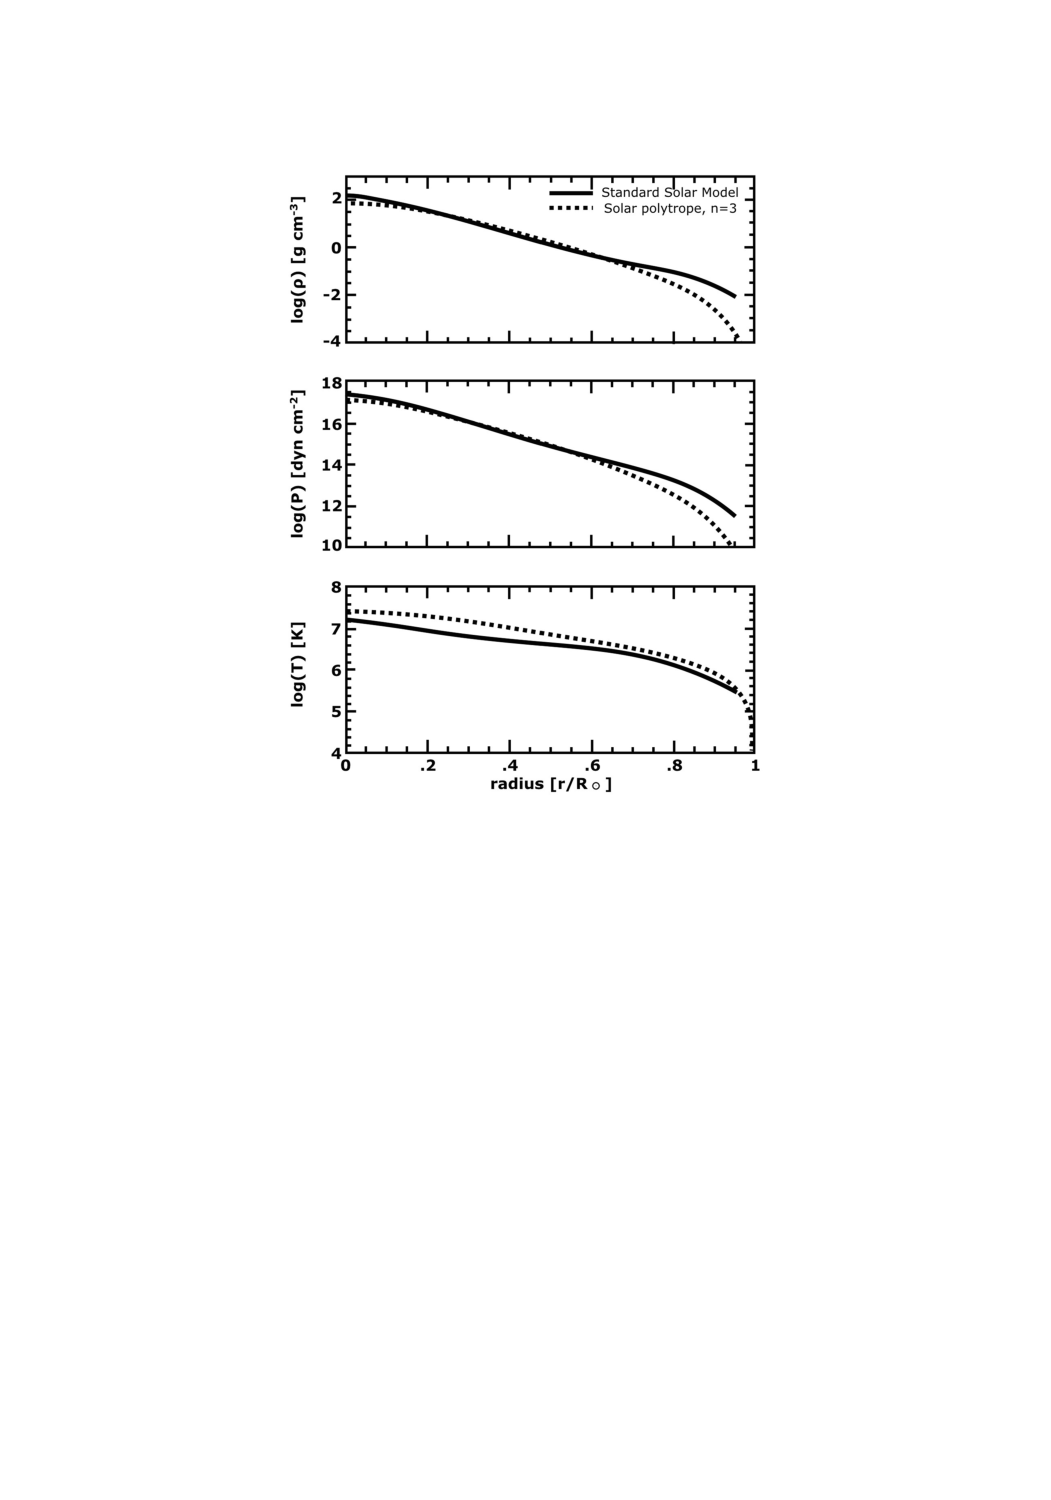
\includegraphics{radiation/figs/eddington-model}
  \caption{The Eddington Model with parameters appropriate for the Sun compared to the Standard Solar Model. (From Lamers \& Levesque.)}
  \label{f.eddington}
\end{figure}

Using the numerical solutions for an $n=3$ polytrope we found in \ref{s.LE-solution}, we can construct a simple Eddington solar model.
In Figure \ref{f.eddington} such a model is shown and compared to a ``Standard Solar Model'' as one might construct using, e.g., MESA.
The comparison is surprisingly good, given the assumptions of the model.
Things go off-the-rails a bit at the edge of the model, but this is to be expected as the assumption of the constant $\beta$ {\it must} breakdown there.
Furthermore, the Eddington model can be used to derive several important relations for main sequence stars (see below and the Exercises).
Incredibly, the Eddington model makes {\it no} assumptions about the source of the energy generation in the star!
Only that the the star is in hydrostatic and radiative equilibrium, which is enough to tightly couple the emergent luminosity with the internal luminosity.


\begin{exercisebox}[Radiation $\beta$ in the Eddington standard model]
Derive an expression for $\beta$ in terms of the mass of the star for the Eddington Standard Model.
\end{exercisebox}

Why is it at all reasonable to take $\beta$ as being constant? To explore this, go back to the equation for radiative diffusion
\[ F(r) = -\frac{1}{3}\frac{c}{\rho\kappa}\frac{\dif aT^{4}}{\dif r}. \]
Write the flux as $F(r) = L(r)/(4\pi r^{2})$, and since pressure decreases monotonically with radius, write
\[
\frac{\dif aT^{4}}{\dif r} = \frac{\dif aT^{4}}{\dif P}\frac{\dif P}{\dif r} = -\rho\frac{Gm(r)}{r^{2}}\frac{\dif aT^{4}}{\dif P}.
\]
The equation of radiation transport then becomes
\[ L(r) = \frac{4\pi Gm(r) c}{\kappa(r)} \frac{\dif P_{\mathrm{rad}}}{\dif P}. \]
Dividing both sides by $L\cdot M/\kappa_{\mathrm{Th}}$ and rearranging terms,
\begin{equation}\label{e.Prad-P}
 \frac{\dif P_{\mathrm{rad}}}{\dif P} = \left[\frac{L\kappa_{\mathrm{Th}}}{4\pi GMc}\right]\left(\frac{\kappa(r)}{\kappa_{\mathrm{Th}}}\frac{L(r)}{L}\frac{M}{m(r)}\right).
\end{equation}
Here $L$ is the total luminosity of the star and $M$ is the total mass.  The term in $[\,]$ is a constant (the Thomson opacity $\kappa_{\mathrm{Th}}$ doesn't depend on density or temperature) and we define the \emph{Eddington luminosity} as $L_{\mathrm{Edd}}=4\pi GM c/\kappa_{\mathrm{Th}}$.  For the sun, $L_{\mathrm{Edd}} = 1.5\ee{38}\nsp\ergs\usp\second^{-1} = 3.8\ee{4}\nsp L_{\sun}$.  For the term $(\,)$ on the right-hand side, note the $L(r)/m(r)$ is basically the average energy generation rate interior to a radius $r$.  Since nuclear reactions are temperature sensitive, the heating is concentrated toward the stellar center and $L(r)/m(r)$ decreases with radius. For stars like the sun, free-free opacity is dominant, and since the free-free Rosseland opacity goes as $T^{-3.5}$, $\kappa(r)$ increases with radius.  Thus, if the energy generation rate is not too temperature dependent (the reaction $\pt + \pt \to \hydrogen[2]$ goes roughly as $T^{4.5}$ at $T=10^{7}\nsp\K$), then the term in $(\,)$  does not vary strongly with radius, and $\dif P_{\mathrm{rad}}/\dif P$ is indeed roughly constant.


\begin{exercisebox}[Dependence of luminosity on stellar mass]
You are now in a position to understand why the luminosity depends strongly on the mass. Cast the flux equation (eq.~[\ref{e.rad-flux}]) into dimensionless form.  Assume the opacity has the functional form $\kappa = \kappa_{0} \rho^{a} T^{-b}$, and scale $\rho$ and $T$ in terms of $M$ and $R$.

\begin{enumerate}
\item You should be able to find a characteristic scale for the luminosity which depends on the stellar mass $M$ and radius $R$, as well as on the exponents $a$ and $b$. Regard $\kappa_{0}$ as a fitting constant, and adjust it so that you get an expression in the form
\[
	\frac{L}{\Lsun} = \left(\frac{M}{\Msun}\right)^{\alpha} \left(\frac{R}{\Rsun}\right)^{\beta}.
\]

\item If the opacity is dominated by Thomson scattering, what are $\alpha$ and $\beta$?  What about if the opacity is Kramer's (eq.~[\ref{e.kramers-opacity}])?
\end{enumerate}
\end{exercisebox}


\input{radiation/mesa-eddington}


\chapter{Transport in a Plasma}\label{ch.plasma-transport}
\input{plasma/plasma}

\chapter{The Initial Mass Function}\label{ch.IMF}
\input{initial-mass-function/initial-mass-function}

\chapter{Contraction to the Main Sequence}
\input{PMScontraction/PMScontraction}

\chapter{Convection}\label{s.convection}
% !TEX root = ../stellar-notes.tex

Hot air rises, as a glider pilot or hawk can tell you. The fluid velocities in question are very subsonic, so we have hydrostatic equilibrium to excellent approximation. But the fluid motions make an enormous difference for heat transport! This state of fluid motions induced by a temperature gradient is known as \emph{convection}. You can perform the following demonstration of the onset of convection.  Brew tea, and pour the hot tea into a saucepan that is on an unlit burner.  Use a straw with your thumb over the top to insert a layer of cold milk under the warm tea in the saucepan.  The temperature difference between the tea and milk will inhibit their mixing. Light the burner, and watch for the development of convection---you will know it when you see it.

\begin{figure}[htbp]
\includegraphics[width=0.5\linewidth]{convection-1}\includegraphics[width=0.5\linewidth]{convection-2}
\caption{Onset of convection in a tea-milk mixture.\label{f.tea}}
\end{figure}

\section{Criteria for onset of convection}\label{s.convection-onset}

To understand this process, let's consider a fluid in planar geometry and hydrostatic equilibrium,
\begin{equation}
\frac{\dif P}{\dif r} = -\rho g.
\end{equation}
Now, imagine moving a blob of fluid upwards from $r$ to $r+h$.  We move the blob slowly enough that it is in hydrostatic equilibrium with its new surroundings, $P_{b}(r+h) = P(r+h)$, where the subscript $b$ refers to ``blob.'' We do move the blob quickly enough, however,  that it does not remain in \emph{thermal} equilibrium with its surroundings; that is, we move the blob \emph{adiabatically}.  The entropy of the blob is therefore constant,
$S_{b}(r+h) = S_{b}(r) = S(r)$, and is therefore not, in general, equal to the entropy of the surrounding gas at $r+h$: $S_{b}(r+h)  \neq S(r+h)$.

As the blob rises, it displaces some of the surrounding fluid. Archimedes tells us that if the displaced fluid is less massive than the blob, then the blob will sink.  We can rephrase this in terms of the volume occupied by a unit mass of fluid $V$: if the volume occupied by the blob is less than the volume of an equal mass of background, then the blob will sink. Translating this into an equation: if
\begin{eqnarray}
\lefteqn{V[P(r+h),S(r+h)] - V_{b}[P_{b}(r+h),S_{b}(r+h)] =}\nonumber\\
&&  V[P(r+h),S(r+h)] - V[P(r+h),S(r)] > 0
\label{e.archimedes}
\end{eqnarray}
then the blob will sink. If condition (\ref{e.archimedes}) is violated, the blob will continue to rise, and the system is unstable to convection.
Figure~\ref{f.convective-schematic} has a cartoon of this process.

\begin{marginfigure}
\includegraphics[width=\textwidth]{convective}
\caption[Illustration of criteria for convective instability.]{\label{f.convective-schematic}Illustration of criteria for convective instability.  On the left, raising a blob a distance $h$ adiabatically and in pressure balance with its surrounding results in a higher density $V_{b} < V$.  This is stable: the blob will sink back.  On the right, the blob is less dense and hence buoyant: it will continue to rise.}
\end{marginfigure}

Taking $h$ to be an infinitesimal displacement and expanding the left-hand side of equation~(\ref{e.archimedes}) gives us a local condition for stability:
\begin{equation}\label{e.convective-stability}
V[P(r+h),S(r)] + \tderiv{V}{S}{P}\frac{\dif S}{\dif r} - V[P(r+h),S(r)]  = \tderiv{V}{S}{P}\frac{\dif S}{\dif r} > 0 .
\end{equation}
Noting that
\begin{eqnarray*}
\tderiv{V}{T}{P} &=& \tderiv{V}{S}{P}\tderiv{S}{T}{P}\\
 &=& \frac{C_{P}}{T}\tderiv{V}{S}{P},
 \end{eqnarray*}
 we can rewrite equation~(\ref{e.convective-stability}) as
 \[
 \frac{T}{C_{P}}\tderiv{V}{T}{P}\frac{\dif S}{\dif r} > 0.
 \]
Now, $(\partial V/\partial T)_{P}$ is positive (gas expands on being heated), so our condition for stability is simply
 \begin{equation}\label{e.entropy-condition}
\frac{\dif S}{\dif r} > 0.
\end{equation}
In a convectively stable star, the entropy must increase with radius. if $\dif S/\dif r < 0$, then convection occurs and carries high-entropy material outward, where it will eventually mix with the ambient medium.  As a result, convection drives the entropy gradient toward the marginally stable configuration $\dif S/\dif r = 0$.  If a star is fully convective and mixes efficiently, then the interior of the star lies along an adiabat.

\newthought{We can derive a condition for convective stability} in terms of the local gradients of temperature and pressure. Writing $S = S[P(r),T(r)]$ we expand equation~(\ref{e.entropy-condition}) to obtain
\begin{equation}\label{e.schwarzschild-1}
\frac{\dif S}{\dif r} = \tderiv{S}{P}{T} \frac{\dif P}{\dif r} + \tderiv{S}{T}{P}\frac{\dif T}{\dif r} .
\end{equation}
Now, $P$ is a monotonically decreasing function of $r$, which means we can use it as a spatial coordinate and write,
\begin{equation}\label{e.TPstar}
\frac{\dif T}{\dif r} = \TPstar \frac{\dif P}{\dif r} .
\end{equation}
Here $\dif T/\dif P|_{\star}$ is the slope of the $T(P)$ relation \emph{for the stellar interior}.  In particular, this is \emph{not} a thermodynamic equality. Substituting equation~(\ref{e.TPstar}) into equation~(\ref{e.schwarzschild-1}), using hydrostatic equilibrium to eliminate $\dif P/\dif r$, and recognizing that $(\partial S/\partial T)_{P} = C_{P}/T$, we obtain
\begin{equation}\label{e.schwarzschild-2}
\frac{\dif S}{\dif r} =  -\rho g\left[\tderiv{S}{P}{T} + \frac{C_{P}}{T} \TPstar \right].
\end{equation}
Finally, we can use the identity (see Appendix~\ref{s.thermo-derivatives})
\begin{equation}
\tderiv{S}{P}{T}\tderiv{T}{S}{P}\tderiv{P}{T}{S} = -1
\end{equation}
to simplify equation~(\ref{e.schwarzschild-2}),
\begin{eqnarray}
\frac{\dif S}{\dif r} &=& -\frac{\rho g}{P}C_{P}\left[\frac{P}{T}\TPstar - \frac{P}{T}\tderiv{T}{P}{S}\right]\nonumber \\
 & = & -\frac{\rho g}{P}C_{P}\left[\nabla - \nablaad\right].
 \label{e.schwarzschild}
\end{eqnarray}
Here we have introduced the shorthand notation $\nabla\equiv \dif \ln T/\dif\ln P|_{\star}$ and $\nablaad \equiv \left(\partial \ln T/\partial\ln P\right)_{S}$.
\emph{A mixture of uniform composition is unstable to convection if the local temperature gradient is steeper than an adiabat, i.e., if $\nabla > \nablaad$.}

\begin{exercisebox}[Temperature as a function of pressure in radiative/convective regions]
Assuming that $\nabla \approx \nablaad$ in a convective region, sketch a plot of temperature as a function of pressure for the following cases.
\begin{enumerate}
\item A star with a stable inner layer and a convective outer layer;
\item A star with a convective inner layer and and a stable outer layer.
\end{enumerate}
Indicate on both of these plots an adiabat.
\end{exercisebox}

\section{A second look at convective instability}\label{s.convection-second-look}

Here we'll take a second-look at the convection by imagining we have a background state with velocity $\vu=0$; we then \emph{perturb} this state by displacing fluid elements a distance $\delta\vr$, and obtaining an equation of motion for $\delta\ddot{\vr}$.  This requires a bit of careful thought on what we are perturbing.

\begin{marginfigure}
\includegraphics[width=\linewidth]{eulerian}
\caption{\label{f.eulerian-grid-1} An Eulerian perturbation: we compare fluid quantities at corresponding locations.}
\end{marginfigure}
There are two types of perturbations. We may change a fluid quantity $f$ at a fixed location $\vr$ and time $t$ (Fig.~\ref{f.eulerian-grid-1}):
\begin{equation}\label{e.eulerian-perturbation}
  \Delta f \equiv f(\vr,t)-f_{0}(\vr,t),
\end{equation}
where the subscript ``0'' denotes the unperturbed quantity.  We call $\Delta f$ an \emph{Eulerian perturbation}.

We may also change a fluid quantity $f$ for a given fluid element; the position of this fluid element in the perturbed system is not necessarily at the same position as in the unperturbed case, however (Fig.~\ref{f.lagrangian-grid-1}):
\begin{equation}\label{e.lagrangian-perturbation}
 \delta f \equiv f(\vr,t) - f_{0}(\vr_{0},t).
\end{equation}
We call $\delta f$ a \emph{Lagrangian perturbation}.
\begin{marginfigure}
\includegraphics[width=\linewidth]{lagrangian}
\caption{\label{f.lagrangian-grid-1} A Lagrangian perturbation: we compare fluid quantities for corresponding fluid elements.}
\end{marginfigure}

Since the fluid element is displaced $\delta\vr = \vr-\vr_{0}$, we can add and subtract $f_{0}(\vr,t)$ to eq.~(\ref{e.lagrangian-perturbation}) and expand $f_{0}(\vr,t)$ to first order in $\delta \vr$ to obtain a relation between the two types of perturbations:
\begin{equation}\label{e.perturbation-relation}
\delta f = \Delta f + (\delta\vr\vdot\grad)f_{0}.
\end{equation}
There are a few useful commutation relations that are easily proved:
\begin{eqnarray}
\partial_{t}\Delta f &=& \Delta\left(\partial_{t}f\right),\\
\grad \Delta f &=& \Delta \grad f,\\
\frac{\Dif}{\Dif t}\delta f &=& \delta \frac{\Dif f}{\Dif t}.
\end{eqnarray}
And there are operations that do not commute:
\begin{eqnarray}
\partial_{t}\delta f &\neq& \delta\left(\partial_{t}f\right),\\
\grad \delta f &\neq& \delta \grad f,\\
\frac{\Dif}{\Dif t}\Delta f &\neq& \Delta \frac{\Dif f}{\Dif t}.
\end{eqnarray}
One can further show that $\delta\vu = (\Dif/\Dif t)\delta \vr$. Finally if the fluid has unperturbed velocity $\vu = 0$, then $\Delta \vu = \delta \vu$.

\newthought{Armed with these relations, let us perturb the momentum equation} by adiabatically displacing a fluid element a distance $\delta\vr$.  We will do this in such a way that the pressure at a fixed location does not change, i.e., $\Delta P = 0$. Of course, the pressure and density of a given fluid element will change according to the relation
\[
\frac{\delta P}{P} = \Gamma_{1}\frac{\delta\rho}{\rho}
\]
with $\Gamma_{1} \equiv \left(\partial \ln P/\partial\ln\rho\right)_{s}$.
We'll also assume that the gravitational force does not change, $\Delta g = 0$.  Our perturbed momentum equation then becomes
\[
\frac{\Dif^{2}\delta\vr}{\Dif t^{2}} = -\frac{1}{\rho + \Delta \rho}\grad P+ \bvec{g}.
\]
Since in the unperturbed fluid $\grad P = \rho\bvec{g}$, this equation simplifies to
\begin{equation}\label{e.perturbed-momentum}
\frac{\Dif^{2}\delta\vr}{\Dif t^{2}} = \frac{\Delta \rho}{\rho}\bvec{g}.
\end{equation}
Expanding,
\begin{eqnarray*}
\frac{\Delta \rho}{\rho} &=& \frac{\delta \rho}{\rho} - \frac{1}{\rho}(\delta\vr\vdot\grad)\rho = \frac{1}{\Gamma_{1}}\frac{\delta P}{P} - \frac{1}{\rho}(\delta\vr\vdot\grad)\rho\\
 &=& \frac{1}{\Gamma_{1}}\frac{\Delta P}{P} + (\delta\vr\vdot\grad)\left[\frac{1}{\Gamma_{1}}\ln P-\ln \rho\right].
\end{eqnarray*}
Since by assumption $\Delta P = 0$, the radial component of equation (\ref{e.perturbed-momentum}) becomes
\begin{equation}\label{e.blob-eq-of-motion}
\delta\ddot{\vr} = g\left[ \frac{\dif\ln\rho}{\dif r} - \frac{1}{\Gamma_{1}}\frac{\dif\ln P}{\dif r} \right] \,\delta r
	\equiv g \mathcal{A} \delta r.
\end{equation}
The quantity $\mathcal{A}$ is called the \emph{Schwarzschild discriminant}: if $\mathcal{A} < 0$, then the motion is oscillatory with frequency $N = (-g\mathcal{A})^{1/2}$; $N$ is called the \emph{Brunt-V\"ais\"al\"a} frequency. The condition $\mathcal{A} > 0$ implies that the fluid is convectively unstable; and indeed, one can show that $\mathcal{A} > 0$ is equivalent to $\dif S/\dif r < 0$\marginnote{The utility of using $\mathcal{A}$ rather than $\dif S/\dif r$ is that $\rho$ and $P$ appear in the equations of stellar structure.}.

\section{Efficiency of Heat Transport}\label{s.efficiency-convection}

A superadiabatic temperature gradient, $\nabla > \nablaad$, induces convective motions. A rising blob will be hotter than its surroundings and heat will therefore be conducted from the blob to its surroundings as it rises. The efficiency by which the heat is transported determines by how much convection is able to drive the temperature gradient towards an adiabat. Clearly the gradient must be super-adiabatic to drive the convection in the first place. We shall see, however, that in stars the difference between the gradient and the adiabat are typically exceedingly small. In other words, convection is extraordinarily efficient at transporting heat.

To understand this, let's go back to equation~(\ref{e.perturbed-momentum}).  Write $\Delta\rho$ as stemming from differences in temperature between rising and falling blobs (recall that $\Delta P=0$).   With this substitution, we have
\begin{equation}\label{e.perturbed-navier-stokes}
 (\partial_{t}\vu + \vu\vdot\grad\vu) = \frac{\Delta\rho}{\rho}\vg = \left(\frac{\partial\ln\rho}{\partial\ln T}\right)_{P}\frac{\Delta T}{T}\vg.
 \end{equation}
%Heat conduction follows the equation
%\begin{equation}\label{e.heat-conduction}
%\rho C_{p}(\partial_{t} + \vu\cdot\grad)T = -\divr \bvec{F} = K\nabla^{2} T
%\end{equation}
%where $K$ is the effective thermal conductivity (includes contributions from both radiative and electronic transport of heat).
Our goal is to estimate the velocity of convective motions $\vu$, the departure of the temperature gradient from an adiabat $\Delta T$, and the fraction of the total heat flux carried by convective motions from these equations.

First, the velocity.  The left-hand side of equation~(\ref{e.perturbed-navier-stokes}) has a characteristic scale $\sim U^{2}/L$, whereas the right-hand side has a scale $g\Delta T/T$. (Recall that in an ideal gas, $(\partial\ln \rho/\partial\ln T)_{P} = -1$.)  If we take $L \sim c_{s}^{2}/g$, a pressure scale height, than we get an estimate of the convective velocity,
\begin{equation}\label{e.convective-velocity-estimate}
\frac{U}{c_{s}} \sim \left(\frac{\Delta T}{T}\right)^{1/2}.
\end{equation}
What is the heat flux carried by convection? Hot fluid rises and carries an excess of heat, per gram, of $c_{P}\Delta T$, giving a heat flux $\approx \rho \vu c_{P}\Delta T$. Thus to carry a given flux $F$, we have
\begin{equation}\label{e.convective-flux-estimate}
c_{s}\rho c_{P} T\left(\frac{\Delta T}{T}\right)^{3/2} \sim F.
\end{equation}
Note that in order of magnitude, $c_{P}T \sim c_{s}^{2}$, so
\[
\frac{U}{c_{s}} \sim \left(\frac{\Delta T}{T}\right)^{1/2} \sim \left(\frac{F}{\rho c_{s}^{3}}\right)^{1/3}.
\]
For conditions in the solar interior, $F \ll \rho c_{s}^{3}$, and therefore the convective velocities are very subsonic. Indeed,
\begin{eqnarray*}
 \frac{F}{\rho c_{s}^{3}} &\sim& \frac{L_{\sun}}{4\pi \Rsun^{2}}\frac{4\pi \Rsun^{3}}{3\Msun}\left(\frac{\Rsun}{G\Msun}\right)^{3/2}\\
  &\sim& \frac{L_{\sun}}{G\Msun^{2}/\Rsun}\left(\frac{\Rsun^{3}}{G\Msun}\right)^{1/2} \\
 	&\sim& \frac{t_{\mathrm{dyn}}}{t_{\mathrm{KH}}} \ll 1.
\end{eqnarray*}
That is, the ratio of the solar flux to what could be carried for near-sonic convective motions is of the order of the dynamical timescale to the Kelvin-Helmholtz timescale.
We therefore expect that in a convective region, slow circulation will produce a temperature gradient that is very nearly adiabatic. This argument breaks down near the surface, where the cooling time of a fluid layer (the ``local'' Kelvin-Helmholtz timescale) can be small.

\section{Turbulence}

From the discussion of the previous section, it might seem possible, given the boundary conditions, of solving for the flow planform, that is, the velocity profile $\vu(\vx,t)$. This is decidedly not the case, however: the flow is turbulent, with intermittent velocity fluctuations seen over a large dynamical range of spatial and temporal scales. Modeling of such flows is a vexing problem in fluid dynamics.

To explore this topic a bit further, we need to introduce the concept of dynamical similarity.  Suppose you want to optimize a wing shape for an aircraft, and you wish to test its performance in a wind tunnel.  Why should you expect that the behavior of a model wing will have any relation to the full-scale one?

To see how this works, start with the Navier-Stokes equation (for simplicity, we'll keep it in one dimension):
\begin{equation}\label{e.navier-stokes-with-visc}
	(\partial_{t} + u\cdot\partial_{x})u = -\frac{1}{\rho}\partial_{x}P + \nu \partial_{x}^{2}u.
\end{equation}
Here $\nu$ is the coefficient of kinematic viscosity, with dimensions $[\nu]\sim [\textrm{length}]^{2}\cdot [\textrm{time}]^{-1}$.
Let's recast equation~(\ref{e.navier-stokes-with-visc}) into dimensionless form by scaling our variable: let $L$ and $U$ represent the characteristic length and velocity scales, and define the dimensionless variables $\tilde{x} = x / L$ and $\tilde{u} = u / U$. This choice then implicitly defines the time variable, $\tilde{t} = t\cdot U/L$. Upon changing to the variables $\tilde{x}$, $\tilde{u}$, and $\tilde{t}$, and writing the equation of state as $P = c_{s}^{2} \rho$ (appropriate for adiabatic flow---we are ignoring heat conduction), we obtain the equation
\begin{equation}\label{e.scaled-NS}
	(\partial_{\tilde{t}} + \tilde{u}\cdot\partial_{\tilde{x}})\tilde{u} = -\left\{\frac{c_{s}^{2}}{U^{2}}\right\}\partial_{\tilde{x}}\ln\tilde{\rho} + \left\{\frac{\nu}{UL}\right\} \partial_{\tilde{x}}^{2}\tilde{u}.
\end{equation}
Each term in this equation is dimensionless.  The physical characteristics of the fluid and the scales involved are described by just two dimensionless parameters:
\begin{eqnarray*}
 \Ma\equiv\frac{U}{c_{s}}&\qquad& \textrm{Mach number (measure of compressibility)}\\
 \Rey\equiv \frac{UL}{\nu} &\qquad& \textrm{Reynolds number (measure of viscous forces)}
\end{eqnarray*}
So, if we build a model wing at a certain scale and place it in a wind tunnel with a certain velocity, then by adjusting the density and temperature (and hence the sound speed and viscosity) to the desired $\Ma$ and $\Rey$, the flow pattern in our model will faithfully replicate the flow in the actual system.

For stellar  convection, $\Ma\ll 1$. What about \Rey?  In typical astrophysical plasmas, the large lengthscales make \Rey\ ludicrously large. Terrestrial experiments and simulations cannot approach this regime. Experimentally, when $\Rey \gtrsim 10^{3}$, then flow becomes \emph{turbulent}: the velocity has strong intermittent fluctuations across a wide range of lengthscales and timescales.  How to characterize the flow in such a case? It is useful to describe the flow in terms of correlated velocities---an ``eddy''---which have some lengthscale.

\begin{marginfigure}
\includegraphics[width=\textwidth]{turbulence-maker}
\caption[A simple mechanism for generating turbulence.]{\label{f.turbulence} A simple mechanism for generating turbulence. A flow of water in a pipe (upstream velocity $U$) flows through a mesh (spacing $L$).  If $\Rey = UL/\nu$ is sufficiently large, the downstream flow becomes turbulent. }
\end{marginfigure}

Suppose we pass water through a pipe that has an embedded mesh screen (Fig.~\ref{f.turbulence}).  For sufficiently large $\Rey = UL/\nu$, where $L$ is the mesh spacing, the downstream flow becomes turbulent. The turbulent eddies are damped.  Now an eddy of size $\lambda$ has an effective Reynolds number $\Rey(\lambda) = U(\lambda)\lambda/\nu$; if this is very large, then molecular viscosity cannot be the reason for damping fluid motions on that scale. Instead what happens is that an eddy with lengthscale $\lambda$ and velocity scale $U(\lambda)$ drives eddies on a smaller scale $\lambda' < \lambda$. These in terms drive still smaller eddies, which in turn drive still smaller eddies, and so on, until eventually very tiny eddies are excited, with size $\lambda_{\nu} \sim \nu/U(\lambda_{\nu})$; and these eddies \emph{are} damped by viscosity!

Kolmogorov argued that in steady-state, intermediate-sized eddies (i.e., those with lengthscales $\nu/U(\lambda) \ll \lambda \ll L$) are neither losing or gaining energy and hence were transferring energy to smaller scales at the same rate as they were being driven; further, this rate at which energy is being transferred to smaller scales is just the net rate of dissipation in the fluid (which is done by the smallest eddies).  The huge dynamic range in lengthscales implies that the velocity of the eddy should not depend on either $L$ or $\nu$, and hence $U(\lambda)$ can only be a function of $\lambda$ (length) and the rate of energy dissipation per unit mass $\varepsilon$ ($\mathrm{energy/mass/time}\sim\mathrm{length^{2}/time^{3}}$). There is only one way to combine these quantities to form something with a dimension of length/time, and so
\begin{equation}\label{e.kolmogorov-velocity}
U(\lambda) \sim \varepsilon^{1/3}\lambda^{1/3}.
\end{equation}
This is seen experimentally: in flows with a large dynamic range of scales, the velocity spectrum follows a power-law with this slope, over an intermediate range of scales, the \emph{inertial range}.  A good example is the flow in a tidal channel\cite{Grant1962Turbulence-spec}.

% Ledoux criterion
%
% Mixing length Theory
%
% Semi-convection
%
% Overshoot
%
% Thermohaline 
\input{convection/mesa-convection}


\chapter[Equation of State]{The Equation of State}\label{ch.equation-of-state}
\input{eos/eos}

\chapter{Nuclear Physics}
% !TEX root = ../stellar-notes.tex

The lives (and deaths) of stars are largely concerned with the history of the nuclear burning they undergo.
Following the gravitational collapse of a protostar and the subsequent contraction to the main sequence (see Chapter \ref{ch.star-formation}), nuclear reactions involving the transmutation of H into He will provide sufficient energy input to balance the radiative luminosity from the stellar surface.
The star will reach radiative and hydrostatic equilibrium. Or at least, nearly so.
This phase, during which a star processes H into He, will the the longest of any phase of stellar evolution, lasting for the Sun some 10 Billion years.
This time scale is quite accelerated for more massive stars as they consume their H fuel at incredibly rapid rates, as we shall see in subsequent chapters.

In order understand how nuclear burning plays a key role in stellar evolution, we must develop some basic knowledge of nuclear physics and nuclear reactions.
This then will provide the final key piece of the puzzle that is the equations of stellar structure (Chapter \ref{ch.equation-of-state}), the elusive local source term due to nuclear reactions $q$.
We shall first describe the basic terminology and definition used to describe nuclear reactions.
Then we will discuss the nuclear landscape and binding energies.
We will then proceed to computing non-resonant reaction cross sections and rates.
After that, we will discuss all important resonant reactions.
Following a brief presentation of computing inverse reaction rates, we will proceed to how reaction rates need be modified to account for important plasma effects.
Finally, we will discuss how all of these rates are folded into systems of differential equations describing the evolution of composition and attendant energy release.

Many excellent and ``classic'' references are available on these topics that go into far greater detail than we will be able.
Perhaps the most ``classic'' (yet still useful...) reference is \cite{Clayton1983Principles-of-S}.
A good exposition of nuclear reactions and networks, and their role in stellar evolution, can be found in \cite{arnett:1996}.
More modern, and slightly experimental, takes can be found in \cite{Iliadis2007Nuclear-Physics}.
And the chapter on nuclear energy generation in \cite{Hansen2004Stellar-Interio} is also a useful summary of the key aspects.

% \begin{enumerate}
%   \item Need intro and overview with definitions and nomenclature.
%   \item Need ignition masses, tie to deuterium burning/hydrogen burning and the end of pre-main sequence phase.
%   \item How do we estimate $T_\mathrm{ign}$?
%   \item More on S factor.
%   \item ``Entrance'' channel ``Exit'' channel
%   \item Branching ratios
% \end{enumerate}

\section{Nuclear Nomenclature}

Consider a reaction that transmutes two bodies into some other two bodies,
\[i + j \rightarrow k + l. \]
For nuclear reactions we have two key constraints: charge conservation $Z_i + Z_j = Z_l + Z_k$, and baryon number conservation $A_i + A_j = A_l + A_k$.
Reactions must also conserve lepton number, so we need to keep track of electrons, positrons, neutrinos, etc.
We define the {\it reaction rate} $r_{ijkl}$ as the number of reactions per second per gram.
The change in energy for the system due to a single such reaction is given by the {\it reaction $Q$-value},
\begin{equation}
  Q_{ijkl} = (m_i + m_j - m_k - m_l) c^2,
\end{equation}
where the term in parentheses is the relativistic change in mass, or {\it mass defect}, of the reaction.
This corresponds to a change in binding energy amongst the nuclei involved.
Finally, the total {\it energy generation rate} for a given reaction is
\begin{equation}
  \epsilon_{ijkl} = r_{ijkl} Q_{ijkl}.
\end{equation}

In nuclear astrophysics, we always consider any complex reaction to be the result of chains of two-body interactions.
Three- and more-body interactions are...complicated.
It is often the case that a give reaction will generate a short-lived, highly-excited compound nucleus that decays so quickly, we typically elide over it's very existence.
For instance, the first step in the proton-proton chain, the primary nuclear fusion going on in the core of Sun, the first reaction is
\[ \mathrm{^1H + ^1H \rightarrow ^2He + e^+} + \nu_e.\]
But in fact, the two protons must first make a $^2$He nucleus.
But this is an incredibly unstable nucleus and so must decay almostly instantly, either back into protons or to deuterium, $^2$H, by the emission of the a positron (and electron neutrino in order to conserve lepton number).

It is common to write nuclear reactions using a shorthand notation, $X(\alpha, \beta)Y$, where the ``target'' nucleus is $X$, the ``projectile'' impacting the target is $\alpha$, and the final nuclear products are $Y$ and $\beta$.
Thus, we would write the proton-proton interaction above as $^1$H($^1$H,e$^+$+$\nu_e$)$^2$He.

Let's consider a more complex reaction, the creation of an excited \carbon nucleus.
The first reaction is proton capture onto \boron
\[ \pt + \boron \rightarrow \carbon^*.\]
This first reaction leading to the excited nucleus is typically called the ``entrance channel'' for the reaction.
This, then, is followed by the decay of the excited carbon nucleus via one of a number of reactions, or ``exit channels:''
\begin{eqnarray*}
  \carbon^* &\rightarrow& \carbon^{**} + \gamma \\
            &\rightarrow& \boron + \pt \\
            &\rightarrow& \carbon[11] + \nt \\
            &\rightarrow& \nitrogen[12] + e^- + \bar{\nu}_e \\
            &\rightarrow& \beryllium[8] + \alpha,\ \mathrm{etc.}
\end{eqnarray*}
The first reaction is simply the generation of some different excited state via the emission of a gamma-ray photon.
Not all exit channels are equally likely.
The probability that a given decay will occur can be computed by comparing the mean lifetimes for the given states, $\tau_i$.

\begin{figure}[htbp]
  \caption{Binding energy per nucleon.}\label{f.bindingE}
  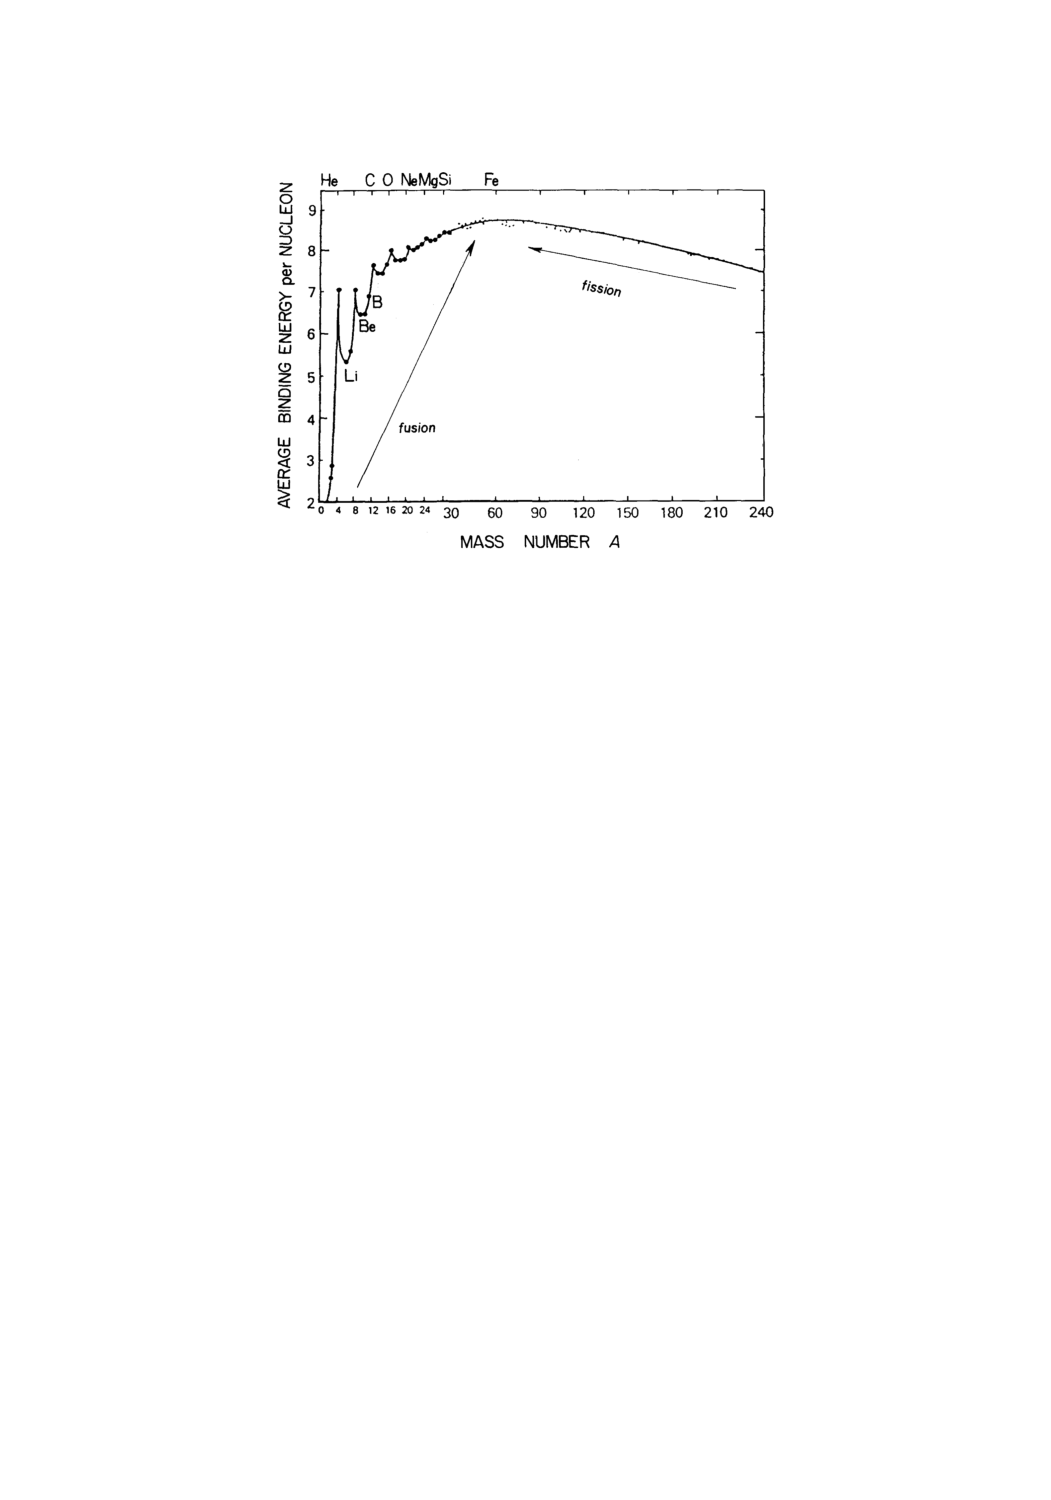
\includegraphics[width=3.5in]{nuclear/figs/bindingE}
\end{figure}

Computing the $Q$ value of a reaction involves comparison the change in binding energy or the the reactants or, equivalently, the mass defect of the reaction.
Figure \ref{f.bindingE} shows the classic, experimentally derived binding energy per nucleon as a function of charge number $Z$.
For example, consider the creation of \carbon via the {\it triple-$\alpha$} reaction,
\[ 3 \helium \rightarrow \carbon. \]
The binding energy per nucleon of the \helium nucleus is 7.074 MeV and that for \carbon is 7.680 MeV.
We can compute the reaction $Q$ value then as
\begin{eqnarray*}
  Q_{3\alpha} &=& 3 \times [4\times (-7.1\ \mathrm{MeV})] - 12\times (-7.7\ \mathrm{MeV}) \\
              &=& -85.2\ \mathrm{MeV} + 92.4\ \mathrm{MeV} = 7.2\ \mathrm{MeV}.
\end{eqnarray*}


\section{The Nuclear Landscape}

From nucleon-nucleon scattering, we find that the nuclear force operates over a range of $\lesssim 2\ee{-13}\nsp\cm \equiv 2\nsp\fermi$, where $\fermi$ denotes the unit of length known as a ``fermi.''  At low energies the nuclear force can be described as the exchange of spin-zero pions; recall from quantum field theory that  the exchange of a spin-zero particle produces an attractive potential of the form $e^{-r/\lambda_{\pi}}/r$, where $\lambda_{\pi} = \hbar/(m_{\pi}c)$ is the Compton wavelength of the force carrier. The pion rest mass is $\approx 140\nsp\MeV/c^{2}$, so $\lambda_{\pi} \approx 1.4\nsp\fermi$.  The nuclear force is indeed attractive over this range,  but it becomes repulsive at distances $< 1\nsp\fermi$ where higher order terms in the interaction become important.

This interaction---short range and attractive, but with a repulsive core---resembles the interaction between molecules in a fluid.  Indeed, for heavy nuclei, the nucleons form a ``nuclear fluid'' with a characteristic density of $0.16\nsp\fermi^{-3}$.  The \textbf{binding energy} is defined as
\begin{equation}\label{e.binding-energy-def}
B(N,Z) = \left[Z m_{p} + N m_{n} - M(N,Z)\right] c^{2},
\end{equation}
where $M$ is the total mass of a nucleus with $N$ neutrons and $Z$ protons. The total number of nucleons is $A = N+Z$, the proton rest mass is $m_{p} = 938.272\nsp\MeV/c^{2}$, and the neutron rest mass is $m_{n} = 939.565\nsp\MeV/c^{2}$.
From the form of this definition $B > 0$ for bound nuclei and is $\approx 8\nsp\MeV$ for most nuclei. This binding of the nucleons into a ``nuclear fluid'' implies that one can make a crude model of the nucleus as a liquid drop, and use this model to fit the binding energy.
Such a model, due to Weiz\"acker, is
\begin{equation}\label{e.weizacker-fmla}
-B(N, Z) = a_{V} A + a_{S}A^{2/3} + a_{A}\frac{(N-Z)^{2}}{A} + a_{C}\frac{Z^{2}}{A^{1/3}} + a_{p}\delta A^{-1/2},
\end{equation}
and has five terms: a bulk energy term $a_{V}A$ that scales with the total number of nucleons; a surface term $a_{S}A^{2/3}$ that corrects for the weaker binding near the surface; an asymmetry term $a_{A}(N-Z)^{2}/A$ that accounts for the energy cost to have an imbalance in the number of neutrons and protons; and a Coulomb term $a_{C}Z^{2}/A^{1/3}$ that accounts for the repulsion between other protons.
 The final term accounts for the pairing between like nucleons, with
\[
\delta = \left\{\begin{array}{lr}+1,& \textrm{$N$, $Z$ even;} \\-1,& \textrm{$N$, $Z$ odd;} \\ 0,& \textrm{$N$ even, $Z$ odd, or $N$ odd, $Z$ even}\end{array}\right. .
\]
A sample fit for the coefficients is listed in Table~\ref{t.liquid-drop-coefficients}.

\begin{table}[htbp]
\caption{Coefficients for the Weiz\"acker mass formula.\label{t.liquid-drop-coefficients}}
\begin{center}
\begin{tabular}{l|rrrrr}
\hline
coefficient & $a_{V}$ & $a_{S}$ & $a_{A}$ & $a_{C}$ & $a_{p}$ \\
\hline\hline
5-parameter fit (MeV) & -15.67 & 17.04 & 23.09 & 0.71 & -14.55\\
4-parameter fit (MeV) & -15.5  &  16.6 & 22.7 & 0.71 & --- \\
\hline
\end{tabular}
\end{center}
\end{table}

\begin{exercisebox}[Is neutron capture endothermic or exothermic?]
In the r-process, a heavy seed nucleus captures a large number of neutrons and then decays back to stability.  Suppose we start with \iron[56] in a bath of free neutrons, so that the iron nucleus captures 152 neutrons (with $\beta$-decays occurring as necessary to keep the nucleus bound) until it reaches the stable nucleus \lead[208].  Is this process exothermic or endothermic? Explain your answer.
\end{exercisebox}

Equation~(\ref{e.weizacker-fmla}) gives a good, if somewhat crude, description of the nuclear landscape.  As a first example,  let's look at how the binding energy per nucleon, $-B/A$ trends with $A$.  For simplicity, we'll ignore the pairing term. Dividing equation~(\ref{e.weizacker-fmla}) by $A$, and denoting the neutron asymmetry by $\eta \equiv (N-Z)/(N+Z)$, we obtain
\begin{equation}\label{e.binding-energy-per-nucleon}
 -\frac{B}{A} = a_{V} + a_{S} A^{-1/3} + a_{A}\eta^{2} + \frac{a_{C}}{4} \left( 1-\eta\right)^{2} A^{2/3}.
\end{equation}
Minimizing this expression for small $A$, we see that the most bound nuclei (smallest $-B/A$) have $\eta \to 0$, i.e., equal numbers of neutrons and protons.  As $A$ increases, however, the Coulomb term becomes important.  Expanding the last two terms and combining gives the sum of the asymmetry and Coulomb terms,
\[ a_{A}\eta^{2} + \frac{a_{C}}{4} \left( 1-\eta\right)^{2} A^{2/3} = \frac{a_{C}}{4} A^{2/3} - \frac{a_{C}}{2}A^{2/3}\eta + \left[ \frac{a_{C}}{4}A^{2/3} + a_{A} \right] \eta^{2} .\]
For large $A$, this expression is minimized (although it cannot be made to vanish) for $\eta > 0$: that is, $N>Z$ and the most bound massive nuclei are neutron-rich. The nuclei for which $-B/A$ is a minimum for a fixed $A$ define the \emph{valley of stability}. How does the binding energy change with $A$ along this valley?  At small $A$, the asymmetry term dominates and $\eta^{2}\ll 1$.  As $A$ increases, the surface term $a_{S}A^{-1/3}$ becomes smaller and $B/A$ increases.  At large $A$, however, the sum of the Coulomb and asymmetry terms decreases $B/A$.  As a result, there is a peak in $B/A$, which is around $A = 56$.

Next, let's find the boundaries of our nuclear landscape: the most neutron-rich and proton-rich nuclei that are still bound.
Define the \textbf{neutron separation energy} $S_{n}$ as the energy needed to remove a neutron from a nucleus,
\begin{eqnarray}\label{e.Sn}
S_{n}(N,Z) &\equiv& c^{2}\left\{\left[M(N-1,Z) + m_{n}\right] - M(N,Z)\right\} \nonumber\\
	&=& B(N,Z) - B(N-1,Z).
\end{eqnarray}
Likewise, define the \textbf{proton separation energy} as
\begin{eqnarray}\label{e.Sp}
S_{p}(N,Z) &\equiv& c^{2}\left\{\left[M(N,Z-1) + m_{p}\right] - M(N,Z)\right\} \nonumber\\
	&=& B(N,Z) - B(N,Z-1).
\end{eqnarray}
If we take a nucleus $(N,Z)$ in the valley of stability and add protons keeping $N$ fixed, we will eventually reach a nucleus for which $S_{p} = 0$, that is, it costs no energy to add or to remove a proton.  This defines the \textbf{proton-drip line}: nuclei more proton-rich are unstable to proton emission. Likewise, on the neutron-rich side there is the \textbf{neutron-drip line}, for which $S_{n} = 0$. Note that because of the pairing term there is an odd-even staggering in the $S_{n}$ and $S_{p}$; it is therefore useful, sometimes, to define the two-neutron and two-proton separations energies $S_{2n}$ and $S_{2p}$.
Figure \ref{f.landscape} shows an annotated nuclear landscape in neutron number and proton number space.

\begin{figure}[htbp]
  \caption{The Nuclear Landscape}\label{f.landscape}
  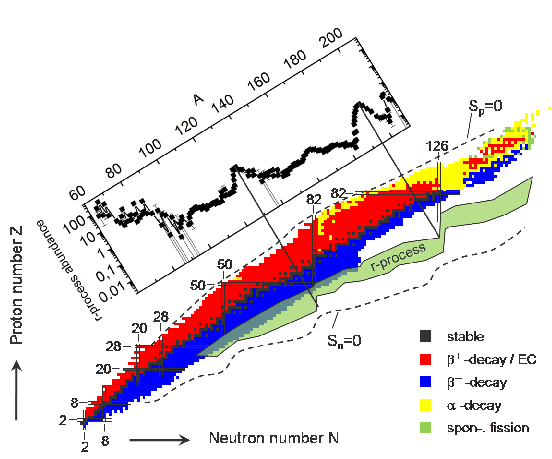
\includegraphics[width=3.5in]{nuclear/figs/landscape}
\end{figure}

\begin{exercisebox}[The nuclear landscape]
\begin{enumerate}
\item
\begin{enumerate}
\item For a fixed $A$, find $Z_\star(A)$ such that the binding energy per nucleon, $f = B(N=A-Z_{\star},Z_{\star})/A$ is maximized.
\item\label{p.one} Plot $Z_{\star}$ vs $N$.
\item Using this $Z_{\star}$, plot $Y_{e}=Z_{\star}/A$ for $20 < A < 200$ and explain qualitatively any trends.
\item Now substitute the value of $Z_{\star}$ into the expression for $B(N,Z)$ and plot $B(N,Z_{\star})/A$ as a function of $A = N + Z_{\star}$. Explain qualitatively any trends.
\end{enumerate}
\item
\begin{enumerate}
\item\label{p.two} For each $10\le Z\le 82$, find the maximum value of $N$ such that $S_{2n}(N,Z) > 0$.  Plot the values $(N,Z)$ you find.
\item\label{p.three} For each $10\le N\le 120$, find the maximum value of $Z$ such that $S_{2p}(N,Z) > 0$. Plot the values $(N,Z)$ you find.
\end{enumerate}

\item Compare the plots of problems \ref{p.one}, \ref{p.two}, and \ref{p.three} to a chart of the nuclides.
\end{enumerate}
\end{exercisebox}

\section{Non-resonant nuclear reactions}

The situation of interest is the reaction between two nuclei, $(A_{1},Z_{1})$ and $(A_{2},Z_{2})$.  The nuclear radius is $\rn\approx  A^{1/3}\nsp\fermi$, and the Coulomb energy at this distance is
\begin{equation}\label{e.cb}
\frac{Z_{1}Z_{2}e^{2}}{\rn} = \frac{Z_{1}Z_{2}\alpha \hbar c}{ \rn} \approx 1.4 Z_{1}Z_{2}A^{-1/3}\nsp\MeV\gg kT.
\end{equation}
For nuclear reactions, typical energy scales  are $\sim\MeV$ and typical length scales are $\sim\fermi$.  In these units, $\hbar c = 197 \nsp\MeV\usp\fermi$.  In the first equality in eq.~(\ref{e.cb}), we also introduce the fine-structure constant $\alpha = e^{2}/(\hbar c) = 1/137$. In ``nuclear units,'' $e^{2} = \alpha \hbar c = (197\nsp\MeV\usp\fermi)/137 = 1.44\nsp\MeV\usp\fermi$. Remember these numbers!  If we scatter two nuclei together, the closest approach (cf.~\S\ref{s.plasma-collisions}) is $\sim e^{2}/(\kB T) \sim 1440\nsp\fermi$ at typical stellar energies $\kB T \sim 1\nsp\keV$.
Clearly the cross-section for a reaction between our pair of particles is controlled by the probability of tunneling through the Coulomb potential.
The situation is illustrated in Figure \ref{f.barrier}.

\begin{figure}[htbp]
  \caption{The Coulomb barrier.}\label{f.barrier}
  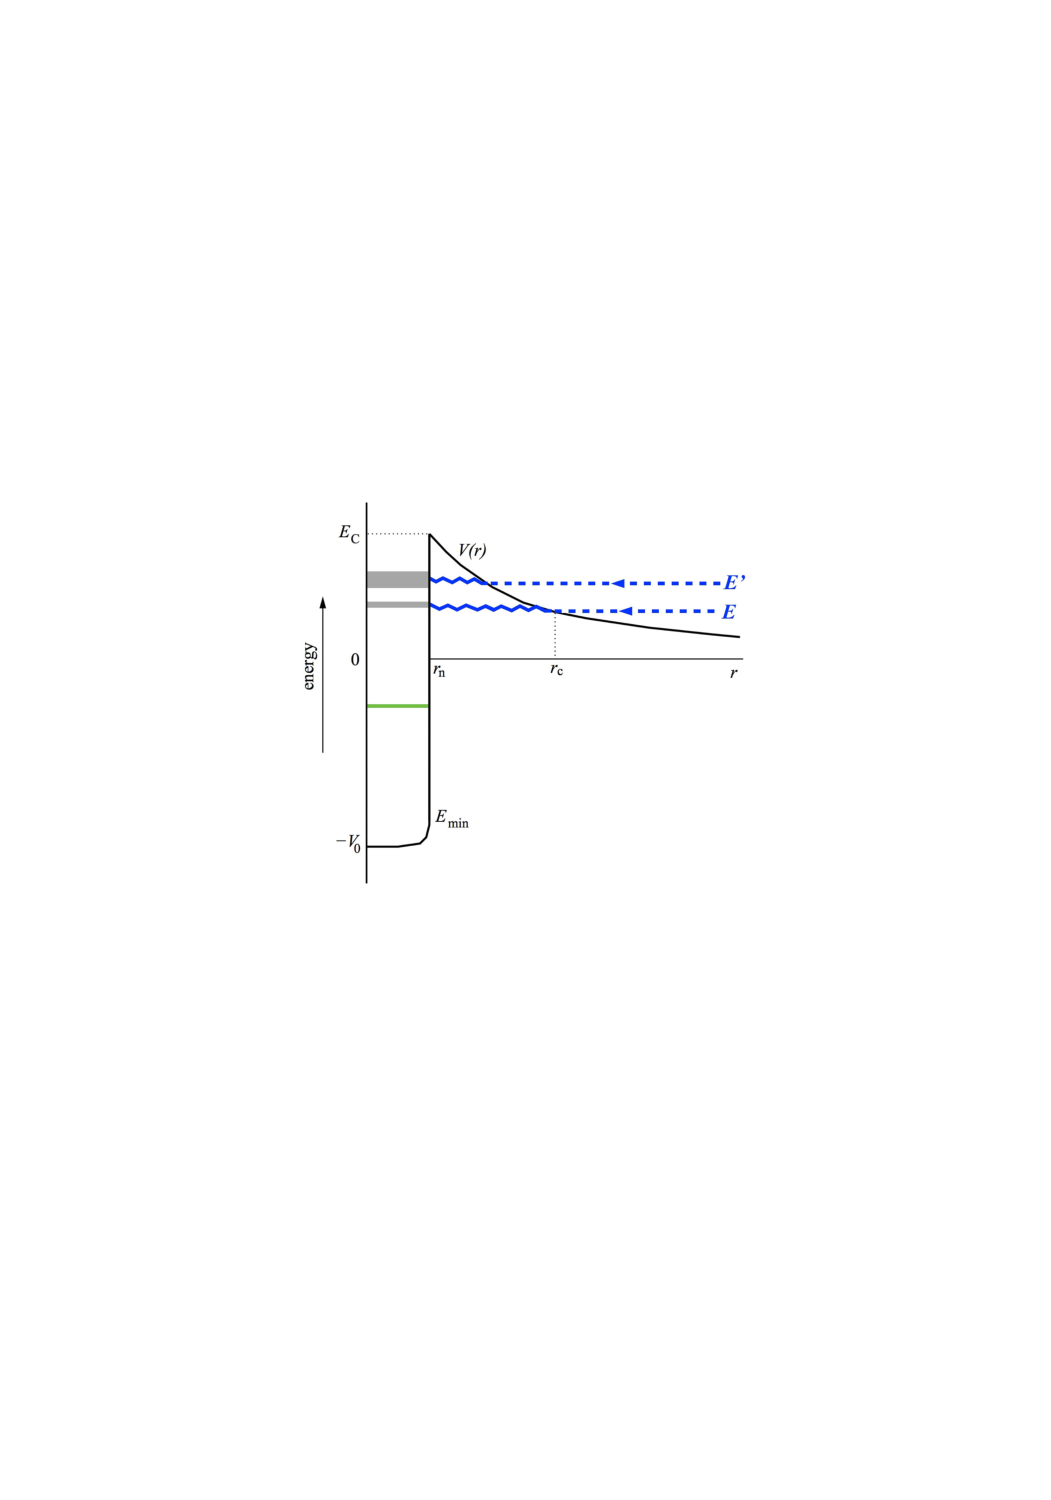
\includegraphics[width=3.5in]{nuclear/figs/potentialWell}
\end{figure}

For a two-body system, it is convenient to transform into a center-of-mass frame.  Our problem then reduces to a one-body problem with reduced mass $m = A\mb$, with $A=A_{1}A_{2}/(A_{1}+A_{2})$ and incident energy $E = m v^{2}/2$, where $v$ is the relative velocity of the two particles.  For now, we'll neglect angular momentum ($\ell = 0$) so our scattering is s-wave.
At low energies, we can form a ``geometrical'' cross-section from the particle wavenumber $k = p/\hbar$, with
\begin{equation}\label{e.geo}
\pi k^{-2} = \pi\frac{\hbar^{2}}{(2mE)} = 660\nsp\barn\frac{1}{A}\left(\frac{\keV}{E}\right)
\end{equation}
Here the cross-section is in units of \emph{barns}, with $1\nsp\barn = 10^{-24}\nsp\cm^{2}$.  This is the first part of our nuclear cross-section $\sigma(E)$.

The second portion of the nuclear cross-section is the probability of tunneling through the Coulomb barrier.  First, let's get the classical turning point \re\ from
\begin{eqnarray}
\frac{Z_{1}Z_{2}e^{2}}{\re} &=& E,\nonumber\\
\re &=& 1440\nsp\fermi\nsp Z_{1}Z_{2}\left(\frac{\keV}{E}\right).
\end{eqnarray}
Now the wavelength is $k^{-1} = \hbar(2A\mb E)^{-1/2} = \hbar c (2A\mb c^{2} E)^{-1/2}$ and since $\mb c^{2} = 932\nsp\MeV$ the wavelength $k^{-1} = 145\nsp\fermi\usp(\keV/E)^{1/2}$. The important point is that since $k^{-1}\ll \re$, we can solve the Schr\"odinger equation using the WKB approximation.

The WKB approximation is standard, so let me just remind you that the probability of tunneling through the barrier depends on the \emph{action},
\begin{equation}\label{e.wkb}
\mathcal{P} \propto \exp\left\{\frac{2}{\hbar}\int_{\re}^{\rn}\left[2m\left(\frac{Z_{1}Z_{2}e^{2}}{r}-E\right) \right]^{1/2}\,\dif r\right\}.
\end{equation}
To do this integral, note that $\re\gg\rn$, so we can make the approximation $\rn\to 0$ in the integral's lower limit; with the substitution
\[
\sin\phi = \left[2m\left(\frac{Z_{1}Z_{2}e^{2}}{r}-E\right) \right]^{1/2}
	\left(\frac{r}{2mZ_{1}Z_{2}e^{2}}\right)^{1/2}
\]
we tame the integral and obtain
\begin{equation}\label{e.prob}
\mathcal{P} \propto \exp\left\{-\frac{8mZ_{1}Z_{2}e^{2}}{\hbar(2mE)^{1/2}}\int_{0}^{\pi/2}\sin^{2}\phi\,\dif\phi\right\} = \exp\left[-\left(\frac{\EG}{E}\right)^{1/2}\right],
\end{equation}
where
\begin{equation}\label{e.EGamow}
\EG\equiv 2\pi^{2} A \mb c^{2} \alpha^{2} (Z_{1}Z_{2})^{2} = 979\nsp\keV \nsp A (Z_{1}Z_{2})^{2}
\end{equation}
is the \emph{Gamow energy}.  Note the strong dependence on $Z_{1}Z_{2}$: \EG\ determines which reactions can occur at a given temperature. If you stare at the factor multiplying the integral in equation~(\ref{e.prob}), you will see that $\mathcal{P}\propto \exp(-\re/\lambda)$, the exponential of ratio of the width of the forbidden region to the wavelength of the incident particle. This makes intuitive sense.

Now we have the second part of our cross-section, the probability of getting through the Coulomb barrier.  This third part depends on the nuclear interactions.  For non-resonant reactions, this third part does not depend strongly on energy, so it is common to define the \emph{astrophysical S-factor} by writing the cross section as the product $(\textrm{geometrical})\times(\textrm{tunneling})\times(\textrm{nuclear})$,
\begin{equation}\label{e.s-def}
\sigma(E) = \frac{1}{E}\exp\left[-\left(\frac{\EG}{E}\right)^{1/2}\right] S(E).
\end{equation}
It is easier to extrapolate the slowly varying $S(E)$ from lab energies of $> 100\nsp\keV$ down to center-of-mass energies of $\sim \keV$ than it would be to fit the rapidly varying cross-section.

Now each nucleus has a Maxwellian velocity distribution,
\begin{equation}\label{e.maxwell}
n_{1}(\bvec{v}_{1})\,\dif^{3}v = n_{1}\left(\frac{m_{1}}{2\pi kT}\right)^{3/2}\exp\left(-\frac{mv^{2}}{2kT}\right) \,\dif^{3}v,
\end{equation}
and similarly for particle 2.  Let's call a particular nucleus 1 (having velocity $\bvec{v}_{1}$) the target. By definition the cross section is
\[ \frac{\textrm{number of reactions}/\textrm{target}/\textrm{time}}{\textrm{number of incident particles}/\textrm{area}/\textrm{time}},
\]
so to get the number of reactions per target per time we need to multiply $\sigma(E)$ by the number of incident particles per unit area per unit time.  The incident flux is just $n_{2}(\bvec{v}_{2})|\bvec{v}|\,\dif^{3}v_{2}$ where $\bvec{v}=\bvec{v}_{2}-\bvec{v}_{1}$.  Hence the reaction rate per unit volume per unit time between a pair of particles having velocities in volumes $\dif^{3}v_{1}$ and $\dif^{3}v_{2}$ about $\bvec{v}_{1}$ and $\bvec{v}_{2}$ is just
\[
\frac{1}{1+\delta_{12}} n_{1}(\bvec{v}_{1})n_{2}(\bvec{v}_{2})\sigma(E)|\bvec{v}| \,\dif^{3}v_{1}\dif^{3}v_{2}.
\]
The factor $(1+\delta_{12})^{-1}$ is equal to $1/2$ if particles 1 and 2 are identical, and is there to avoid double-counting in that case. To get the total reaction rate per unit time, we need to integrate over the joint velocity distribution $\dif^{3}v_{1}\,\dif^{3}v_{2}$,
\begin{eqnarray}\label{e.rate-joint}
\lefteqn{r_{12} = \frac{n_{1}n_{2}}{1+\delta_{12}}  \left[\frac{m_{1}m_{2}}{(2\pi kT)^{2}}\right]^{3/2}}
  \nonumber\\ &&\times\int\! \sigma(E) v\exp\left(-\frac{m_{1}v_{1}^{2}}{2kT}-\frac{m_{2}v_{2}^{2}}{2kT}\right)  \,\dif^{3} v_{1}\,\dif^{3}v_{2}.
\end{eqnarray}
Now $E$ and $v$ are the relative energies and velocity in the center-of-mass frame.  We can change variable using the relations
\begin{eqnarray*}
\bvec{v}_{1} &=& \bvec{V} - \frac{m_{2}}{m_{1}+m_{2}} \bvec{v}\\
\bvec{v}_{2} &=& \bvec{V} + \frac{m_{1}}{m_{1}+m_{2}} \bvec{v}.
\end{eqnarray*}
where $V$ is the center-of-mass velocity. It is straightforward to show that $\dif v_{1,x}\,\dif v_{2,x} = \dif V_{x}\dif v_{x}$, and likewise for the $y,z$ directions.  Furthermore, $m_{1}v_{1}^{2} + m_{2}v_{2}^{2} = (m_{1}+m_{2})V^{2} + m v^{2}$, and multiplying and dividing the integral in equation~(\ref{e.rate-joint}) by $m_{1}+m_{2}$ allows us to write
\begin{eqnarray*}
\lefteqn{r_{12} = \frac{n_{1}n_{2}}{1+\delta_{12}} \left(\frac{m_{1}+m_{2}}{2kT}\right)^{3/2}\left(\frac{m}{2kT}\right)^{3/2}}\\
&&\times \int\!\dif^{3}V \int\!\dif^{3}v \,\sigma(E)v \exp\left[-\frac{mv^{2}}{2kT}\right]
 \exp\left[-\frac{(m_{1}+m_{2})V^{2}}{2kT}\right].
\end{eqnarray*}
The integral over $\dif^{3}V$ can be factored out and is normalized to unity. Hence we have for the reaction rate between a pair of particles 1 and 2,
\begin{eqnarray}\label{e.rate}
r_{12} &=& \frac{1}{1+\delta_{12}}n_{1}n_{2}\left\{\left(\frac{m}{2\pi kT}\right)^{3/2}\int_{0}^{\infty}\! \sigma(E) v \exp\left(-\frac{mv^{2}}{2kT}\right)  4\pi v^{2}\,\dif v\right\}.\nonumber\\
 &\equiv& \frac{1}{1+\delta_{12}}n_{1}n_{2}\langle\sigma v\rangle.
\end{eqnarray}
The term in $\{\}$ is the averaging over the joint distribution of the cross-section times the velocity, and is usually denoted as $\langle\sigma v\rangle$.

Changing variables to $E = mv^{2}/2$ in equation~(\ref{e.rate}) and inserting the formula for the cross-section, equation~(\ref{e.s-def}), gives
\begin{equation}\label{e.integral}
\langle\sigma v\rangle = \left(\frac{8}{\pi m}\right)^{1/2}\left(\frac{1}{kT}\right)^{3/2}\int_{0}^{\infty}\!S(E)\exp\left[-\left(\frac{\EG}{E}\right)^{1/2}-\frac{E}{kT}\right]\,\dif E.
\end{equation}
Now, we've assumed that $S(E)$ varies slowly; but look at the argument of the exponential. This is a competition between a rapidly rising term $\exp[-(\EG/E)^{1/2}]$ and a rapidly falling term $\exp(-E/kT)$. As a result, the exponential will have a strong peak, and we can expand the integrand in a Taylor series about the maximum. Let
\[
f(E) = -\left(\frac{\EG}{E}\right)^{1/2} - \frac{E}{kT}.
\]
Then we can write
\begin{eqnarray*}
\lefteqn{\int_{0}^{\infty}\!S(E)\exp\left[-\left(\frac{\EG}{E}\right)^{1/2}-\frac{E}{kT}\right]\,\dif E}\\
&\approx&
	\int_{0}^{\infty}\! S(\Epk)\exp\left[f(\Epk) + \frac{1}{2}\left.\frac{\dif^{2} f}{\dif E^{2}}\right|_{E=\Epk}\left(E-\Epk\right)^{2}\right].
\end{eqnarray*}
Here $\Epk$ is found by solving $(\dif f/\dif E)|_{E=\Epk} = 0$. This trick allows us to turn the integral into a Gaussian! (Before the internet, all there was to do for fun were integrals.)

Solving for \Epk, we get
\[
\Epk = \frac{\EG^{1/3}(kT)^{2/3}}{2^{2/3}},
\]
and
\[ \exp\left[f(\Epk)\right] = \exp\left[-3\left(\frac{\EG}{4kT}\right)^{1/3}\right].
\]
Further,
\[
\left.\frac{1}{2}\frac{\dif^{2}f}{\dif E^{2}}\right|_{E=\Epk} = -\frac{3}{2(2\EG)^{1/3}(kT)^{5/3}} = -\frac{3}{4\Epk kT}.
\]
Defining a variable $\Delta = 4(\Epk kT/3)^{1/2}$, our integral becomes
\begin{eqnarray}\label{e.integral2}
\lefteqn{\langle\sigma v\rangle = \left(\frac{8}{\pi m}\right)^{1/2}\left(\frac{1}{kT}\right)^{3/2}}\nonumber\\
&&\times S(\Epk)
  \exp\left[-3\left(\frac{\EG}{4kT}\right)^{1/3}\right]
  \int_{0}^{\infty}\!\exp\left[-\frac{(E-\Epk)^{2}}{(\Delta/2)^{2}}\right]\,\dif E.
\end{eqnarray}
How well does this approximation do?  Figure~\ref{f.integrand} shows the integrand (\emph{solid line}) and the approximation by a Gaussian (\emph{dashed line}).  Although the integrand is skewed to the right, the area is approximately the same.  We could correct for this by taking more terms in our expansion. Consult Clayton for details.

\begin{figure}[htbp]
\includegraphics[width=4in]{coulomb_integrand}
\caption[Competition between Boltzmann factor and penetration of Coulomb barrier in setting the thermally-averaged reaction rate.]{Integrand of eq.~(\protect\ref{e.integral}) (\emph{solid line}) and the Gaussian (\emph{dot-dashed line}) constructed by expanding to second order the argument of the exponential. The parameters for $\EG$ were taken from the $p+p$ reactions ($Z_{1}Z_{2}=1$, $A = 1/2$), and the temperature is $10^{7}\nsp\K$.  Note that the grey curves, showing the two terms of the exponential, have been rescaled to fit on the same plot.}
\label{f.integrand}
\end{figure}

Another simplification can be made because both the Gaussian and the original integrand go to zero as $E\to 0$.  As a result, we can extend the lower bound of our integral (eq.~[\ref{e.integral2}]) to $-\infty$, and obtain
\begin{eqnarray}\label{e.rate2}
\langle\sigma v\rangle &\approx& \left(\frac{8}{\pi m}\right)^{1/2}\left(\frac{1}{kT}\right)^{3/2} S(\Epk) \exp\left[-3\left(\frac{\EG}{4kT}\right)^{1/3}\right]\frac{\Delta}{2}\nonumber\\
 &=& \frac{2^{13/6}}{\sqrt{3m}}\frac{\EG^{1/6}}{(kT)^{2/3}} \exp\left[-3\left(\frac{\EG}{4kT}\right)^{1/3}\right]  S(\Epk).
\end{eqnarray}
On to some numbers. Table~\ref{t.reaction} lists quantities for some common reactions. A couple of notes. First, $\Delta/\Epk$ indicates how well our Gaussian approximation works---you will see it is less than 1 in all cases. We evaluated $\Delta/\Epk$, which decreases with temperature as $T^{-1/6}$, at $T = 10^{7}\nsp\K$. Second, the quantity $n(T)$ is the exponent if we want to approximate the reaction rate as a power-law, $r\propto T^{n}$.  We compute this as
\begin{equation}\label{e.exponent}
 n(T) = \frac{\dif\ln r}{\dif\ln T} = -\frac{2}{3} + \left(\frac{\EG}{4kT}\right)^{1/3},
 \end{equation}
 as you can easily verify for yourself. In the table, the exponent is evaluated at $T = 10^{7}\nsp\K$; obviously $n$ depends on temperature. Finally, note the size of $\EG/(4k)$.  This makes the argument of the exponential in equation~(\ref{e.rate2}) large in absolute value, and sets the temperature scale at which a given reaction comes into play.

\begin{table}[htbp]
\caption{\label{t.reaction} Parameters for non-resonant reactions}
\begin{center}
\begin{tabular}{lrrrrrr}
\hline
Reaction & $p+p$ & $p+\helium[3]$ & $\helium[3]+\helium[3]$ & $p+\lithium[7]$ & $p+\carbon$\\
\hline\hline
$A$ & 1/2 & 3/4 & 3/2 & 0.88 & 0.92 \\
$Z_{1}Z_{2}$ & 1 & 2 & 4 & 3 & 6 \\
$\EG$ (MeV) & 0.489 & $2.94$ & $23.5$ & $7.70$ & $32.5$\\
$\EG/(4k)$ (GK) & $1.4$ & $8.5$ & $68.0$ & $22.0$ & $94.0$ \\
$\Epk|_{T=10^{7}\nsp\K}$ (keV) & 4.5 & 8.2 & 16.3 & 11.3 & 18.2\\
$\Delta/\Epk|_{T=10^{7}\nsp\K}$ & 1.0 & 0.75 & 0.53 & 0.64 & 0.50 \\
$n(T = 10^{7}\nsp\K)$ & 4.6 & 8.8 & 18.3 & 12.4 & 20.5\\
\hline
\end{tabular}
\end{center}
\end{table}
%
%Once we have the reaction rate per pair of particles, the volumetric heating rate for the reaction $a+X$ is then
%\begin{equation}\label{e.heating-rate}
%\rho\varepsilon = Q\frac{n_{a}n_{X}}{1 + \delta_{aX}}\langle \sigma v\rangle.
%\end{equation}
%Now, $n_{a} = Y_{a}\rho/\mb$, where $Y_{a} = X_{a}/A_{a}$ is the abundance ($X_{a}$ is the mass fraction), and likewise for $n_{X}$. The denominator $1+\delta_{aX}$ takes care of double-counting if $a$ and $X$ are identical.

\section{Resonances}\label{s.resonant-reactions}

This section contains my condensed notes on resonances following Blatt and Weisskopf's excellent text\cite{Blatt1979Theoretical-Nuc}.  Other treatments of the subject, such as that in Iliadis\cite{Iliadis2007Nuclear-Physics} and in Clayton\cite{Clayton1983Principles-of-S}, mostly follow their approach. In this section, we shall often make use of the notation $X(a,b)Y$ to mean the reaction $X + a \to b + Y$.

\subsection{Orbitals}
Nuclei exhibit shell effects: one can often treat the nucleons as independent particles occupying orbitals determined by a mean force.  Unlike in the atomic case, the spin-orbit term in the Hamiltonian, $-a\bvec{L}\vdot\bvec{S}$, is quite strong. Since the total angular momentum is $\bvec{J}=\bvec{L}+\bvec{S}$, we have
\[
\bvec{L}\vdot\bvec{S} = \frac{1}{2}\left(\bvec{J}\vdot\bvec{J} - \bvec{L}\vdot\bvec{L} - \bvec{S}\vdot\bvec{S}\right),
\]
and hence states with larger $\bvec{J}$ have a lower energy. The strong $\bvec{L}\vdot\bvec{S}$ coupling leads to the presence of ``gaps'' in the energy spectra; nuclei that have have filled (either neutrons or protons) shells up to this gap are unusually bound and the nucleon number (either neutron or proton) is termed a \emph{magic number}. The magic numbers are 2, 8, 20, 28, 50, 82, and 126. For example, \oxygen\ (8 protons, 8 neutrons) and \calcium\ (20 protons, 20 neutrons) are doubly magic and hence more strongly bound than other nuclides of similar mass.

We label the orbitals as $n\ell_{j}$, where $n$ is the radial quantum number, $\ell$ is the orbital angular momentum ($s,p,d,f,\ldots$), and $j$ is the total angular momentum.  The first few orbitals are listed in Table~\ref{t.orbitals}.  Each orbital has $2j+1$ nucleons, and a fully occupied orbital has $\bvec{J}=0$. For example, we would expect that the ground state of \carbon[13] (6 protons, 7 neutrons) to have closed $1s_{1/2}$ and $1p_{3/2}$ shells for both neutrons and protons, and the remaining neutron would then occupy the $1p_{1/2}$ shell.

\begin{table}[htbp]
\caption{\label{t.orbitals} Neutron orbitals}
\begin{center}
\begin{tabular}{ccc}
\hline
Orbital & Number, $2j+1$, in orbital & Total number\\
\hline\hline
$1d_{3/2}$ & 4 & 20\\
$2s_{1/2}$ & 2 & 16\\
$1d_{5/2}$ & 6 & 14\\
$1p_{1/2}$ & 2 & 8\\
$1p_{3/2}$ & 4 & 6\\
$1s_{1/2}$ & 2 & 2\\
\hline
\end{tabular}
\end{center}
\end{table}

The remaining quantum number is parity ($\bvec{\pi}$), which is conserved under the strong force. The parity of a nucleon orbital is $(-1)^{\ell}$, where the angular momentum number $\ell$ must be summed over all nucleons. Since a closed shell has an even number of nucleons, it must have positive parity. For example, the ground state of $\oxygen[17]$ has 8 protons filling the $1s_{1/2}$, $1p_{3/2}$, and $1p_{1/2}$ shells 8 neutrons in closed shells, so the remaining neutron must be in the  $1d_{5/2}$ shell ($\ell=2$): the angular momentum and parity of the ground state must therefore be $j^{\pi} = \frac{5}{2}^{+}$. As a second example, \nitrogen has 6 protons in closed shells and 6 neutrons in closed shells, with the remaining proton and neutron both in $1p_{1/2}$ orbitals.  Hence the angular momentum of the ground state could either be $0$ or $1$; it turns out that the symmetric state has lower energy, so $j=1$. The parity of the ground state is $(-1)^{1 + 1} = 1$, so $J^{\pi}( \nitrogen) = 1^{+}$.

The angular momentum matters because it sets the possible range of relative angular momenta that the incoming particles can have.  Writing the wave function as $\psi(r) = (u_{\ell}(r)/r)Y_{\ell 0}$ and substituting  into Schr\"odinger's equation,
\[
-\frac{\hbar^{2}}{2m}\nabla^{2}\psi + V(r)\psi  = E\psi,
\]
gives the following equation for $u_{\ell}$,
\[
\frac{\dif^{2}}{\dif r^{2}} u_{\ell} + \left\{ k^{2} - \frac{\ell(\ell + 1)}{r^{2}} - \frac{2m}{\hbar^{2}}\frac{Z_{a}Z_{X}e^{2}}{r} \right\}u_{\ell} = 0.
\]
Here $k$ is the wavenumber for the particle at $r\to\infty$, $E = \hbar^{2}k^{2}/2m$. Note the presence of the ``centrifugal barrier,''
\[ \frac{\hbar^{2}}{2mr^{2}} \ell(\ell+1)  = 20.9\nsp\MeV\frac{\mb}{m}\left(\frac{\fermi}{r}\right)^{2}\ell(\ell+1): \]
there is a price to pay if the particles must have a high relative $\ell$.

\subsection{Formation of a compound nucleus}
Even orbitals with positive energy can be long-lived; suppose we excite a proton in \carbon[11] to an orbital just above the threshold for decay into $\pt + \boron[10]$.  Although this state has positive energy and can decay, the particle has to tunnel through the coulomb barrier, and potentially an angular momentum barrier if $s$-wave emission is forbidden.  We saw that the probability of getting through the Coulomb barrier (for $s$-wave) is given by eq.~(\ref{e.prob}).  If this is very small, then we can imagine a classical particle oscillating back and forth in the well, which is does many times because the probability of escaping each time it approaches the barrier is so small. Thus, if there is a substantial energy barrier impeding escape, the classical oscillation period $P$ is much less than the lifetime of the state $\tau$.  Now the classical oscillation period depends inversely on the spacing $D$ between energy levels, $P \sim \hbar/D$, as you can verify for an infinite square well potential.  Hence if the probability of tunneling is sufficiently small,
\[
 \frac{P}{\tau} \sim \frac{\hbar}{D\tau} = \frac{\Gamma}{D} \ll 1,
\]
where the width of the state to particle emission is $\Gamma = \hbar/\tau$.  Hence for reactions at low excitation energies involving light nuclei with widely separated levels, we can look at captures into discrete levels in the compound nucleus.

\subsection{Derivation of resonant cross-section}\label{s.resonant-cross-section}
We're now ready to do some heavy lifting and derive the cross-section for a resonant reaction.  The nuclear force is short-ranged, so we can define a ``channel radius'' $R$ exterior to which our potential is purely Coulomb. Our strategy is just like doing transmission resonances in quantum mechanics: we'll solve for the wave function exterior to $R$ and match it to the wave function inside $R$.  Since we don't completely know the form of the potential inside $R$, our expression will have terms that must be experimentally constrained.

The reaction is $a + X$; the coulomb potential is $Z_{a}Z_{X}e^{2}/r$ and the relative angular momentum of $a$ and $X$ is $\ell$.  Let $m$ be the reduced mass of $a$ and $X$.  Our wave function is then $\psi(r) = (u_{\ell}(r)/r)Y_{\ell 0}$; substituting this into the Schr\"odinger equation,
\[
-\frac{\hbar^{2}}{2m}\nabla^{2}\psi + V(r)\psi  = E\psi,
\]
gives the following equation for $u_{\ell}$,
\[
\frac{\dif^{2}}{\dif r^{2}} u_{\ell} + \left\{ k^{2} - \frac{\ell(\ell + 1)}{r^{2}} - \frac{2m}{\hbar^{2}}\frac{Z_{a}Z_{X}e^{2}}{r} \right\}u_{\ell} = 0.
\]
Here $k$ is the wavenumber for the particle at $r\to\infty$, $E = \hbar^{2}k^{2}/2m$. There are two solutions to this differential equation; the solutions are known as Coulomb wave functions, $F_{\ell}$ and $G_{\ell}$.  The regular solution $F_{\ell}$ vanishes as $r\to 0$, and $G_{\ell}$ blows up at the origin.
For $kr \gg 1$, the Coulomb wave functions go over to
\begin{eqnarray}\label{e.coulombF}
F_{\ell}(r) &\simeq& \sin\left[ kr - \frac{1}{2}\ell\pi -\gamma\ln(2kr) + \sigma_{\ell}\right]\\
G_{\ell}(r) &\simeq& \cos\left[ kr - \frac{1}{2}\ell\pi -\gamma\ln(2kr) + \sigma_{\ell}\right].
\label{e.coulombG}
\end{eqnarray}
Here the parameter $\sigma_{\ell}$ is a Coulomb phase shift, and the parameter
\[ \gamma = \frac{1}{2\pi}\left(\frac{E_{G}}{E}\right)^{1/2} \]
contains the Gamow energy.  This shouldn't be too surprising: since $F_{\ell}$ and $G_{\ell}$ are the exact solutions to the motion of a particle in a Coulomb potential, they must behave like what we found using a WKB approximation in some limit.

For $r \geq R$, we can write our solution in terms of outgoing waves, $u_{\ell}^{+}$, and incoming waves, $u_{\ell}^{-}$; here the outgoing and incoming waves are defined as
\begin{eqnarray*}
u_{\ell}^{+} &=& e^{-i\sigma_{\ell}}\left[G_{\ell} + i F_{\ell}\right]\\
u_{\ell}^{-} &=& e^{i\sigma_{\ell}}\left[G_{\ell} - i F_{\ell}\right].
\end{eqnarray*}
At large distances these go over to plane waves,  and so we can determine the coefficients,
\begin{equation}\label{e.coulomb-solution}
u_{\ell} = \frac{\sqrt{\pi}}{k}i^{2\ell + 1}(2\ell +1)^{1/2}\left[u_{\ell}^{-} - \eta_{\ell}u_{\ell}^{+}\right].
\end{equation}
The effect of the nucleus is to affect the outgoing waves via the coefficient $\eta_{\ell}$.  Furthermore, if we integrate the current over a large sphere we obtain the cross-section for the reaction (if the current is zero, then every particle that enters the sphere leaves it, so there is no reaction),
\begin{equation}\label{e.cross-section-eta}
\sigma_{\ell} = \frac{\pi}{k^{2}}(2\ell +1) \left[ 1 - |\eta_{\ell}|^{2}\right].
\end{equation}
To determine $\eta_{\ell}$, we need to find the logarithmic derivative
\[
\alpha_{\ell} \equiv R\left.\frac{u_{\ell}'}{u_{\ell}}\right|_{r=R}
\]
where $u_{\ell}' = \dif u_{\ell}/\dif r$.  For now $\alpha_{\ell}$ is undetermined, since it depends on the wave function inside the nucleus.  It is useful to define the following quantities:
\begin{eqnarray}\label{e.coulombPhase}
\frac{u_{\ell}^{-}}{u_{\ell}^{+}} & = & \frac{G_{\ell} - i F_{\ell}}{G_{\ell} + i F_{\ell}}e^{2i\sigma_{\ell}} \equiv e^{2i\xi}\\
R\left.\frac{u_{\ell}^{+'}}{u_{\ell}^{+}}\right|_{r=R} &=& R(G_{\ell}'G_{\ell} + F_{\ell}'F_{\ell})v_{\ell} + i kR v_{\ell} \equiv \Delta_{\ell} + is_{\ell}.
\label{e.delta-s}
\end{eqnarray}
In the last equation, we made use of the fact that $G_{\ell}F_{\ell}' - F_{\ell}G_{\ell}' = k$ for all $r$ and defined
\[
v_{\ell} = \left(G_{\ell}^{2} + F_{\ell}^{2}\right)^{-1}_{r=R}.
\]
To see the significance of $v_{\ell}$, note that the ratio of an outgoing wave at $r\to\infty$ and that at $r=R$ is
\[
\frac{|u_{\ell}(\infty)|^{2}}{|u_{\ell}(R)|^{2}} = \frac{1}{G_{\ell}^{2}(R) + F_{\ell}^{2}(R)},
\]
where the numerator follows from the asymptotic forms, eqns.~(\ref{e.coulombF}) and (\ref{e.coulombG}). This ratio, however, is just the probability of the wave transmitting through the potential barrier, and for $\ell=0$ is approximately what we found earlier (eq.~[\ref{e.prob}]) using the WKB approximation.

Evaluating $\alpha_{\ell}$ for the solution defined at $r \geq R$, eq.~(\ref{e.coulomb-solution}), and using our definitions, eq.~(\ref{e.coulombPhase}) and (\ref{e.delta-s}), we determine the phase shift,
\[
\eta_{\ell} = \frac{\alpha_{\ell} - \Delta_{\ell} + is_{\ell} }{\alpha_{\ell} - \Delta_{\ell} -i s_{\ell}}e^{2i\xi}.
\]
Using this to evaluate the reaction cross-section, eq.~(\ref{e.cross-section-eta}), we have
\begin{equation}\label{e.cross-section-alpha}
\sigma_{\ell} = \frac{\pi}{k^{2}}(2\ell +1) \frac{-4s_{\ell}\Im\alpha_{\ell}}{(\Re\alpha_{\ell}-\Delta_{\ell})^{2} + (\Im\alpha_{\ell} - s_{\ell})^{2}}
\end{equation}
Notice that the reaction cross-section vanishes if $\alpha_{\ell}\in\mathbb{R}$, i.e., $\Im\alpha_{\ell}=0$.  So far, our efforts may just look like we are reshuffling terms for no apparent reason, but there is a method to the algebraic madness. We see explicitly, for example, that the cross-section is proportional to the penetration through the term $s_{\ell}$ in the numerator.

To make further progress, we have to evaluate $\alpha_{\ell}$, and this requires making some constraints on the form of the wavefunction at $r < R$. Although the precise form of the potential is unknown, we do know that it is a rather deep well.  Just inside the surface $R$, we expect the radial wavefunction to be composed of spherical waves,
\[
u_{\ell}(r<R) = A\left\{\exp(-iKr) + e^{2i\zeta}e^{-2q}\exp(iKr)\right\}.
\]
Our reasoning for this form is as follows.  In general the state will be a standing wave, which we can write as a sum of incoming and outgoing waves.  The jump in the potential at $r=R$ introduces a phase shift, which we parameterize by $e^{2i\zeta}$. If the state decays by another channel than simply re-emitting the particle, i.e. if a reaction occurrs, then the amplitude of the outgoing wave will be less than that of the incoming wave; we parameterize this by the factor $e^{-2q}$.  We expect that $q\ll 1$, because otherwise the state wouldn't be long-lasting and have a well-defined energy.

We can factor $u_{\ell}(r<R)$,
\begin{eqnarray*}
u_{\ell}(R) &=& \left(2A e^{i\zeta}e^{-q}\right)\left\{\frac{\exp(-iKR -i \zeta + q) + \exp(iKR + i \zeta - q)}{2}\right\} \\
 &=& C\cos(KR+\zeta + iq).
\end{eqnarray*}
Using this to evaluate the logarithmic derivative,
\begin{equation}\label{e.alpha}
\alpha_{\ell} = -KR\tan(KR + \zeta + iq).
\end{equation}
Now, recall that $K \gg k$; the wavenumber inside the nuclear potential well is much larger than that outside.  The only way to smoothly join two waves with such discrepant wavenumbers is to have them match where $u_{\ell}' = 0$, i.e., where $\alpha_{\ell} = 0$.  Let's expand $\alpha_{\ell}$ about such a point with energy $\varepsilon_{r}$ and $q = 0$:
\[
\alpha_{\ell} \approx \left.\frac{\partial\alpha_{\ell}}{\partial \varepsilon}\right|_{q=0,\varepsilon=\varepsilon_{r}}(\varepsilon - \varepsilon_{r}) + \left.\frac{\partial\alpha_{\ell}}{\partial q}\right|_{q=0,\varepsilon=\varepsilon_{r}} q.
\]
Substituting this into equation~(\ref{e.cross-section-alpha}) gives
\begin{equation}\label{e.sigma-penultimate}
\sigma = \frac{\pi}{k^{2}}(2\ell+1)\left\{\frac{ 4KRq s_{\ell}}{[(\partial_{\varepsilon}\alpha_{\ell})(\varepsilon - \varepsilon_{r}) - \Delta_{\ell}]^{2} + [ -KRq - s_{\ell}]^{2}}\right\}.
\end{equation}
We expect that near a resonance, the cross-section will have a Lorentzian profile, with a total width
\[
\Gamma = \sum_{i}\Gamma_{i} + \Gamma_{\gamma}
\]
that is the sum of particle decay widths $\Gamma_{i}$ and widths for radiative transitions $\Gamma_{\gamma}$.  The entrance channel width will be proportional to $s_{\ell}=kRv_{\ell}$. Furthermore, a reaction will take place if the nucleus does something other than decay in the entrance channel, and this will occur with probability $\Gamma - \Gamma_{a}$.

Motivated by these considerations, we note that
if we define the width for decay in the entrance channel as
\begin{equation}\label{e.Gamma-entrance}
\Gamma_{a} = -\frac{2s_{\ell}}{\partial_{\varepsilon}\alpha_{\ell}} = -\frac{2kR\,v_{\ell}}{\partial_{\varepsilon}\alpha_{\ell}},
\end{equation}
the reaction width as (it can be shown that in general $\partial_{\varepsilon}\alpha_{\ell} < 0$)
\begin{equation}\label{e.Gamma-reaction}
\Gamma_{r} = \Gamma-\Gamma_{\alpha} = -\frac{2KR\,q}{\partial_{\varepsilon}\alpha_{\ell}},
\end{equation}
and the ``observed'' resonance energy as
\[
\varepsilon_{r,\mathrm{obs}} = \varepsilon_{r} + \frac{\Delta_{\ell}}{\partial_{\varepsilon}\alpha_{\ell}},
\]
then the cross-section becomes
\begin{equation}\label{e.breit-wigner}
\sigma = \frac{\pi}{k^{2}}(2\ell + 1)\frac{\Gamma_{a}\Gamma_{r}}{(\varepsilon - \varepsilon_{r,\mathrm{obs}})^{2} + (\Gamma/2)^{2}}.
\end{equation}
This is the cross-section for a compound nucleus to form in channel $a$ and decay by any other channel.  To get the cross-section for a specific exit channel $b$, we must multiply by the branching ratio $\Gamma_{b}/\Gamma_{r}$.  Finally, for an unpolarized incident beam, we need to multiply the cross section by a statistical factor
\begin{equation}\label{e.stat-factor}
\omega = \frac{2J + 1}{(2J_{a}+1)(2J_{X}+1)}
\end{equation}
to account for the fraction of angular momentum states in the target $X$ and beam $a$ that can enter the level with the appropriate angular momentum $\ell$.

You might be troubled by our identification of the particle width, eq.~(\ref{e.Gamma-entrance}), and reaction width, eq.~(\ref{e.Gamma-reaction}). Notice that if we were to solve the problem of a quasi-bound state leaking out of its well, we would encounter similar equations, and this would lead to the identification of the level width.  We can make the argument more plausible by the following consideration.  Let's consider $\partial_{\varepsilon}\alpha_{\ell}$, evaluated about the point where $\alpha_{\ell} = 0$ and $q= 0$.  The general form of $\alpha_{\ell}$ is a tangent function (eq.~[\ref{e.alpha}]), so if we increase the energy by the spacing between levels $D$, the phase of the tangent must increase by $\pi$.  Hence, $\partial_{\varepsilon}\alpha_{\ell}|_{KR + \zeta = n\pi, q=0} \sim -KR\pi/D$. Substituting this into eq.~(\ref{e.Gamma-entrance}) and rearranging,
\[
\Gamma_{a} \sim \hbar \left(\frac{4k}{K}\right)\left(\frac{D}{2\pi\hbar}\right)v_{\ell}.
\]
Now, when a plane wave is incident on a step in the potential, the transmission coefficient across the step is roughly $k/K$, as you can verify by solving a one-dimensional Schr\"odinger equation.  We saw earlier that classical oscillation period for a particle in a well is $2\pi\hbar/D$. Hence
\begin{eqnarray*}
\lefteqn{\Gamma_{a} \sim \hbar\times(\textrm{oscillation frequency})}\\
&& \times(\textrm{transmission across potential step at nuclear surface})\\
 && \times(\textrm{probability of penetrating coulomb, centrifugal barrier}).
\end{eqnarray*}
But this is precisely what we would write down for $\hbar\times(\textrm{rate of decay in channel $a$})$---the particle has a small probability on each oscillation to penetrate the potential jump and barrier.

\subsection{A worked example}

Consider the reaction $\boron[10](\pt,\alpha)\beryllium[7]$. We can think of this reaction proceeding first via the formation of a compound nucleus in an excited state, $\carbon[11]^{\star}$. It can be shown that the cross-section for the formation of $\carbon[11]^{\star}$ via proton capture is proportional to the width for the decay of that state via proton emission:
\begin{equation}\label{e.reciprocity}
\sigma(\pt + \boron[10]\to \carbon[11]^{\star}) \propto \Gamma_{\pt}.
\end{equation}
The second stage of the reaction is the decay of the $\carbon[11]^{\star}$ into $\alpha + \beryllium[7]$.
Because of the short timescale $\sim 10^{-23}\nsp\second$ for nuclear interactions---roughly the crossing time for a nucleon in a $20\nsp\MeV$ by $2\nsp\fermi$ well---we make the assumption that the decay of an excited state does not depend on how the state was formed. If $\Gamma_{\alpha}$ represents the decay $\carbon[11]^{\star}\to \alpha+\beryllium[7]$, then
\[ \sigma(\pt + \boron[10] \to \alpha+\beryllium[7]) \propto \Gamma_{\pt}\Gamma_{\alpha}. \]
The full expression for the cross section is
\begin{equation}\label{e.resonant-cross-section}
 \sigma(\pt + \boron[10] \to \alpha+\beryllium[7])  = \frac{\pi}{k^{2}}(2\ell + 1)\omega\frac{\Gamma_{\pt}\Gamma_{\alpha}}{(\varepsilon - \varepsilon_{r,\mathrm{obs}})^{2} + (\Gamma/2)^{2}}.
\end{equation}
Here the first term $\pi(2\ell+1)k^{-2}$ is the geometrical cross-section and $\Gamma$ represents the total decay width of the excited state in the compound nucleus.  The factor $\omega$  is the statistical factor
\[
\omega = \frac{2J + 1}{(2J_{\pt}+1)(2J_{10}+1)}
\]
that accounts for the fraction of angular momentum states that can enter the level with the appropriate angular momentum $\ell$.
For our example, the reaction $\boron[10](\pt,\alpha)\beryllium[7]$ can proceed via  the $J^{\pi} = 5/2^{+}$ level at $8.70\nsp\MeV$ in \carbon[11].  The angular momentum and parity of \boron[10] and the proton are $J^{\pi}(\boron[10]) = 3^{+}$, $J^{\pi}(\pt) = 1/2^{+}$.  These two spins can add to either $7/2^{+}$ (multiplicity of 8) or $5/2^{+}$ (multiplicity of 6).  As a result, they can enter into the resonance with $\ell = 0$, and they will do so with $6/14$ probability.  The cross section for this reaction is then
\[
\sigma(\pt + \boron[10]\to\beryllium[7]+\alpha) = \frac{6}{14}\frac{\pi}{k^{2}}\frac{\Gamma_{\pt}\Gamma_{\alpha}}{(\varepsilon-\varepsilon_{8.70})^{2} + (\Gamma/2)^{2}}.
\]
This is multiplied by the entrance channel velocity $v$ and integrated over the thermal distribution to produce the reaction rate.

\section{Inverse Rates}\label{s.inverse-rates}

Consider a photodisintegration reaction $Y(\gamma,a)X$.  We could compute the rate for this by first computing the excitation $Y\to Y^{*}$ by absorption of a photon followed by decay through the $a$-channel.  There is another, easier, way to compute the thermally averaged rate, however, if we already have an expression for the forward reaction $X(a,\gamma)Y$.  Suppose we allow our plasma, consisting of $a$, $X$, and $Y$ to come into thermal balance.  In such a plasma, the composition does not change with time, so our forward and inverse rates must balance:
\begin{equation}\label{e.balanced-rates}
 n_{X}n_{a}\langle \sigma v \rangle_{Xa} = n_{Y}\lambda,
\end{equation}
where $\lambda$ is the photodissociation rate.  Since we are in thermal equilibrium, however, we also have a relation between the chemical potentials,
\[ \mu_{X} + \mu_{a} = \mu_{Y}. \]
For an ideal gas, the chemical potentials are given by eq.~(\ref{e.chem-pot-ideal-gas}). Rearranging terms gives and taking the exponential gives us the equation
\begin{equation}\label{e.Xa-Y}
	\frac{n_{X}n_{a}}{n_{Y}} = \frac{n^{Q}_{X}n^{Q}_{a}}{n^{Q}_{Y}}\exp\left(-\frac{Q}{\kB T}\right).
\end{equation}
In this expression we have substituted $Q = (m_{a}+m_{X}-m_{Y})c^{2}$, and
\[
	n^{Q}_{i} = g_{i}\left(\frac{m_{i}\kB T}{2\pi\hbar^{2}}\right)^{3/2}.
\]
Substituting eq.~(\ref{e.Xa-Y} into eq.~(\ref{e.balanced-rates}) gives us an expression for the photodissociation rate $\lambda$ in terms of the forward rate,
\begin{eqnarray}
 \lambda &=& \frac{n_{X}n_{a}}{n_{Y}} \langle \sigma v \rangle_{Xa} \nonumber\\
 \label{e.inverse-from-balance}
 &=& \frac{g_{X}g_{a}}{g_{Y}} \left(\frac{\mb \kB T}{2\pi\hbar^{2}}\right)^{3/2} \left(\frac{A_{X}A_{a}}{A_{Y}}\right)^{3/2} \exp\left(-\frac{Q}{\kB T}\right) \langle \sigma v \rangle_{Xa}.
\end{eqnarray}
This expression is specific to this type of reaction, but similar formula can be generated for other types of reactions, such as $X(a,b)Y$.

\section{Plasma corrections to the reaction rate}\label{s.correction-penetration}

In stars, the nuclear reactions do not occur in isolation, but rather in the midst of a plasma.  The effect of these ambient charges is to screen the long-range Coulomb interaction. This in turn perturbs the penetration factors and hence the reaction rates. We now derive the lowest order correction \cite{Salpeter1954Electrons-Scree}.

The first thing to consider are the typical scales involved.  In a plasma, the mean interparticle spacing is
\[ a = \left(\frac{3A\mb}{4\pi \rho}\right)^{1/3} = 1.6\ee{4}\nsp\fermi\times A^{1/3}\left(\frac{100\nsp\grampercc}{\rho}\right)^{1/3},
\]
and the Debye length (cf.\ eq.~[\ref{e.linearized-Poisson}]) is
\[
\lambdaD = 2.8\ee{4}\nsp\fermi\times \left(\frac{T}{10^{7}\nsp\K}\right)^{1/2} \left(\frac{100\nsp\grampercc}{\rho}\right)^{1/2} \left(\frac{A}{\langle Z^{2}+Z\rangle}\right)^{1/2}.
\]
Both of these lengths, for typical conditions in a stellar plasma, are much larger than the size of the classically forbidden region through which the particle must tunnel: at $\Epk = 10\nsp\keV$, this length is $\re = 144\,Z_{1}Z_{2}\nsp\fermi \ll a < \lambdaD$.  The nuclear scale is $\sim\fermi$ and is much smaller that all of these.

The penetration factor (eq.~[\ref{e.wkb}]) depends on the potential in the barrier; given that $\re \ll \lambdaD$, we may expand the potential, eq.~(\ref{e.screened-potential}), and write
\begin{equation}
\mathcal{P} \propto \exp\left\{\frac{2}{\hbar}\int_{\re}^{\rn}\left[2m\left(\frac{Z_{1}Z_{2}e^{2}}{r} - \frac{Z_{1}Z_{2}e^{2}}{\lambdaD} - E\right) \right]^{1/2}\,\dif r\right\}.
\end{equation}
Since $\lambdaD$ doesn't depend on either $E$ or $r$, the effect of the screening potential is just to  change the zero point of the energy scale.  Assuming the $S$-factor doesn't depend sensitively on energy, the effect of screening on the rate is just to multiply the integrand in equation~(\ref{e.rate}) by
\begin{equation}\label{e.fscreening}
  f_{\mathrm{scr}} = \exp\left(\frac{Z_{1}Z_{2}e^{2}}{\lambdaD\kB T}\right).
\end{equation}
Since this factor doesn't depend on $E$, it simply multiplies the rate $\langle\sigma v\rangle$.  Note that since $\lambdaD > a$ and since $e^{2}/(a\kB T) \ll 1$ in a plasma, this screening factor is a small correction to the rate.

\section{Equations for Chemical Evolution}\label{e.eqns-for-chem-evol}

Now that we have a reaction cross-section, we can write down the equations describing the chemical evolution of the star, and the nuclear heating. To make this concrete, let's look at the reaction $\pt + \pt \to e^{+}\nu_{e} + \hydrogen[2]$. The reaction rate is (cf.\ eqs.~[\ref{e.rate}] and [\ref{e.fscreening}])
\[ r_{pp} = \frac{1}{2} n_{\mathrm{H}}^{2}f^{\mathrm{scr}}_{pp}\langle\sigma v\rangle_{pp}. \]
Each reaction destroys 2 protons, so we can write down our equation for the change in $n_{\mathrm{H}}$,
\begin{equation}\label{e.H-conservation-1}
\partial_{t} n_{\mathrm{H}} + \divr(n_{\mathrm{H}}\vu) = -n_{\mathrm{H}}^{2} f^{\mathrm{scr}}_{pp} \langle\sigma v\rangle_{pp}.
\end{equation}
Likewise, the $pp$ reaction produces deuterium, which is in turn destroyed by $\mathrm{D} + \pt \to \helium[3]$:
\begin{equation}\label{e.H-conservation-2}
\partial_{t} n_{\mathrm{D}} + \divr(n_{\mathrm{D}}\vu) = \frac{1}{2} n_{\mathrm{H}}^{2} f^{\mathrm{scr}}_{pp}\langle\sigma v\rangle_{pp} - n_{\mathrm{D}} n_{\mathrm{H}} f^{\mathrm{scr}}_{Dp}\langle\sigma v\rangle_{Dp}.
\end{equation}
Let's write each number density in terms of its abundance: $n_{\mathrm{H}} = Y_{\mathrm{H}}\NA\rho$. We can then use the equation of mass continuity (eq.~[\ref{e.mass-1}]) to simplify these equations to
\begin{eqnarray}
\left(\partial_{t} + \vu\vdot\grad\right) Y_{\mathrm{H}}  &=& -Y_{\mathrm{H}}^{2}\rho f^{\mathrm{scr}}_{pp} \left[\NA\langle\sigma v\rangle\right]_{pp}\label{e.H-abund} \\
\left(\partial_{t}  + \vu\vdot\grad\right) Y_{\mathrm{D}} &=& \frac{1}{2} Y_{\mathrm{H}}^{2}\rho f^{\mathrm{scr}}_{pp} \left[\NA\langle\sigma v\rangle\right]_{pp} \nonumber\\ && {}- Y_{\mathrm{D}} Y_{\mathrm{H}} \rho f^{\mathrm{scr}}_{Dp}\left[\NA \langle\sigma v\rangle\right]_{Dp}. \label{e.D-abund}
\end{eqnarray}
The left-hand side of these equations are just the Lagrangian time derivatives. On the right-hand sides, the quantities in $[\,]$ are just functions of temperature and are compiled into rate libraries, such as \textsc{reaclib}.
We will need equations like (\ref{e.H-abund}) and (\ref{e.D-abund}) for each species in our star. A collection of such equations is known as a \textbf{reaction network}.

Each reaction is specified by a $Q$-value, which is just the energy deposited into the gas by the reactions. If there is no neutrino released, this will just be the change in nuclear binding energy, but for reaction like $\pt + \pt$ one has to account for the energy carried off by the neutrino.  For the two reactions we consider here, the total heating rate, per unit mass, is
\begin{eqnarray}
q &=& \frac{1}{\rho}\left(\frac{Q_{pp}}{2}n_{\mathrm{H}}^{2} f^{\mathrm{scr}}_{pp}\langle\sigma v\rangle_{pp} + Q_{DP} n_{\mathrm{D}}n_{\mathrm{H}} f^{\mathrm{scr}}_{Dp}\langle\sigma v\rangle_{Dp}\right)\\
 &=& \frac{Q_{pp}\NA}{2}Y_{\mathrm{H}}^{2}\rho f^{\mathrm{scr}}_{pp} \left[\NA\langle\sigma v\rangle\right]_{pp} \nonumber \\
 && {}+ Q_{Dp}\NA Y_{\mathrm{D}}Y_{\mathrm{H}} \rho f^{\mathrm{scr}}_{Dp} \left[\NA\langle\sigma v\rangle\right]_{Dp} .
\label{e.heating-rate}
\end{eqnarray}
The equations for the change in chemical composition and the heating rate close our system of equations describing the structure and evolution of the star.  We are now ready to discuss the life cycle of stars in detail.


\chapter[Main Sequence]{Hydrogen Burning and the Main Sequence}
\input{main-sequence/main-sequence}

\chapter[Low-Mass Post-Main Sequence]{Post-Main Sequence Evolution: Low-mass Stars}
\input{post-main-sequence/post-main-sequence}

\chapter[Rotation and Magnetic Fields]{Rotation and Magnetic Fields}\label{ch.rotation}
%\input{}

\chapter[Standard Solar Model]{The Standard Solar Model}\label{ch.solarmodel}
%\input{}

\chapter[High-mass Stars]{Evolution of High-mass Stars}\label{ch.highmass}
%\input{}

\chapter[Core-collapse Supernovae]{Core-collapse Supernovae}\label{ch.ccsn}
%\input{}

\chapter{Binaries}\label{ch.binaries}
\input{binaries/binaries}

\chapter[Type Ia Supernovae]{Type Ia Supernovae}\label{ch.rotation}
%\input{}

\chapter{Stellar Pulsations}\label{s.pulsations}
\input{perturbations/perturbations}

\chapter[Stellar Atmospheres]{Stellar Atmospheres}\label{s.stellar-atmospheres}
\input{atmosphere/atmosphere}



\appendix
\chapter{Technical Notes}\label{s.technical-notes}
\input{technical-notes/technical-notes}

\backmatter
\bibliographystyle{plainnat}
\bibliography{bibs/stellar}

\end{document}
